% Nature-format reformat of "Serving Is Learning".
% Single-column Article layout: 200-word summary paragraph, flowing main text
% with short bold run-in headers, Methods, Extended Data, availability
% statements. Quantitative figures come from make_figs.py + make_figs_nature.py
% (house rule: every number from a committed jsonl). Compile: latexmk -pdf main_nature
\documentclass[sn-nature]{sn-jnl}   % official Springer Nature / Nature Portfolio template

\usepackage{graphicx}
\usepackage{booktabs}
\usepackage{amsmath,amssymb,amsfonts}
\usepackage{xcolor}
\usepackage{manyfoot}               % sn-jnl footnote setup expects this in the preamble
\usepackage[font=small,labelfont=bf]{caption}
\DeclareCaptionLabelSeparator{bar}{ \textbar\ }
\captionsetup{labelsep=bar}
\usepackage{tikz}
\usetikzlibrary{arrows.meta,positioning,backgrounds,fit,calc}
% NOTE: sn-jnl loads geometry + hyperref + natbib(sn-nature) itself; do not re-load.

\definecolor{learner}{HTML}{2A78D6}
\definecolor{normc}{HTML}{1BAF7A}
\definecolor{firec}{HTML}{4A3AA7}
\definecolor{yellowc}{HTML}{C98500}
\definecolor{goodc}{HTML}{1B7A3A}

\newcommand{\heading}[1]{\vspace{4pt}\noindent\textbf{#1}\hspace{0.6em}}

\begin{document}

\title[One dynamics for perception and plasticity]{One dynamics for perception
and plasticity: predictive coding that learns as it serves}

\author*[1]{\fnm{Anonymous} \sur{Author}}\email{anon@example.com}
\affil*[1]{\orgname{Anonymous Institution}}

\abstract{Predictive-coding theories cast perception as
continuous inference, in which the brain predicts its input, computes what it
failed to anticipate, and treats learning not as a separate phase but as an
occasional, surprise-gated consequence of the same ongoing
computation\cite{rao1999predictive,friston2010free,keller2018predictive}. However such
predictive coding networks tend to be shallow and constrained to toy problems.
Traditional deep neural networks do the opposite whereby they act, and, in a different process
on different hardware at a different time, they learn---reconciling the two at a
cost in storage, synchronization and energy\cite{espeholt2018impala}. Here we
show that separation is unnecessary. On a tropical predictive coding model,
where assigning credit reduces to re-tracing the winning computation the forward
pass already performed, one process answers every input and, whenever it is
surprised, turns that same computation into an exact learning step---with no
second pass, no stored activations and no multiplication in the reverse sweep.
The result is a concrete, hardware-realizable deep predictive-coding model in which
serving is inference and learning is inference, and
which makes testable predictions about potential cortical credit assignment and
consolidation. We demonstrate running this model persistently on a ten-million-example
lifetime in one process at almost no added cost with bounded forgetting; on
reconfigurable silicon the added power of learning falls below the instrument
floor.}

\keywords{predictive coding, continual learning, on-device learning, tropical
algebra, neuromorphic hardware}

\maketitle

\begin{figure}[t]
\centering
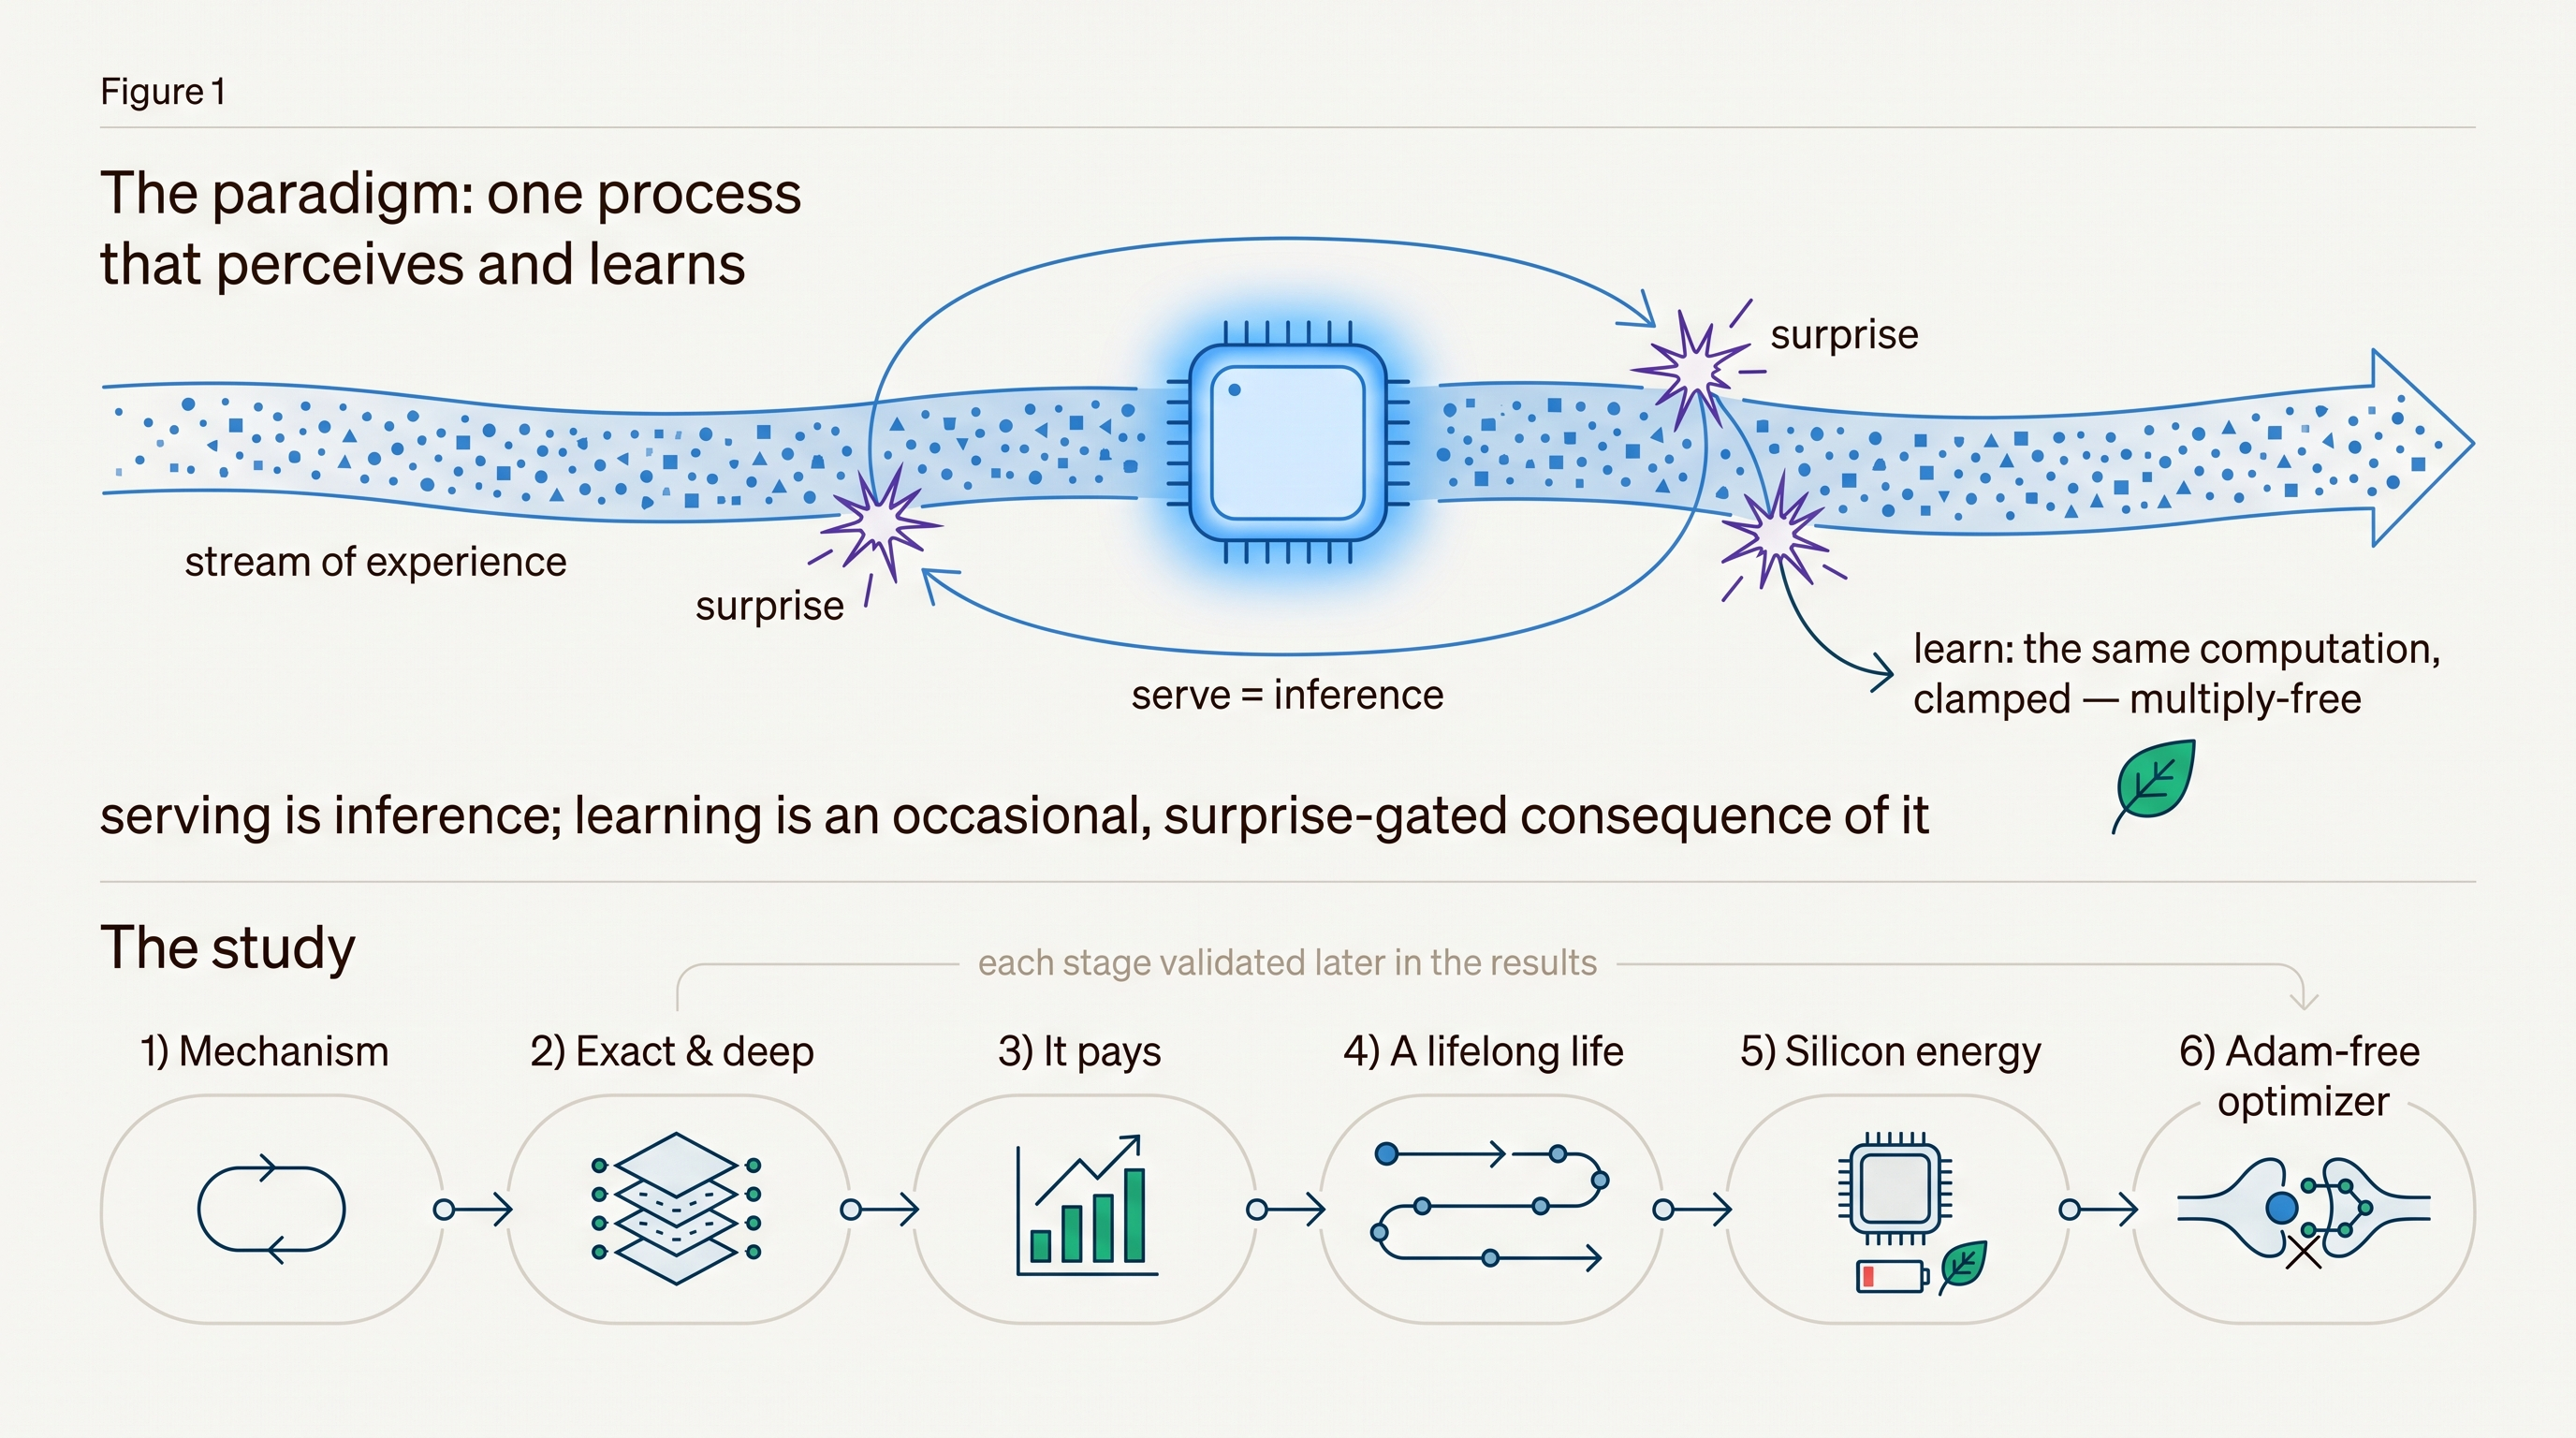
\includegraphics[width=\textwidth]{figs/gen/fig1_hero.jpg}
\caption{\textbf{One process that perceives and learns, and the study.} Top: the
paradigm---a single predictive-coding device sits on its stream of experience;
serving is inference, and whenever it is surprised the same computation becomes an
(occasional, multiply-free) learning step. Bottom: a roadmap of the study---the
mechanism, its exactness and depth, that it pays, a device-scale lifetime, silicon
energy, and a fully closed optimizer---each validated in the results.
\emph{(Design draft; to be redrawn as a vector figure for submission.)}}
\label{fig:paradigm}
\end{figure}

% ======================================================================
% MAIN TEXT
% ======================================================================
In predictive-coding theories, perception is not a feedforward reaction to
stimuli but an ongoing act of inference: a constantly active cortex predicts
its sensory input, propagates the mismatch---the prediction error---up a
hierarchy, and adjusts continuously, with prior expectations and their precision
resolving ambiguity in the incoming signal\cite{rao1999predictive,friston2010free,
keller2018predictive,bastos2012canonical}. Two features of this picture are
pertinent here. First, the brain does not stop acting in order to learn:
plasticity is a local, always-available, energy-gated property of the very
circuits that compute behaviour\cite{fremaux2016neuromodulated,
lillicrap2020backpropagation}, the whole system runs on about twenty
watts\cite{attwell2001energy}, and no organism schedules a backward pass or
maintains a replica of itself for training. Second, ongoing activity is not
idle---the same predictive machinery that serves perception is the machinery
that learns from it, and prior expectations continuously shape what is
perceived\cite{flounders2019neural}. Deployed neural networks make the opposite
choice. Even systems called ``online''---streaming reinforcement learners,
test-time-training models, periodically fine-tuned services---run two
computations: a forward path that produces behaviour, and a training path with
its own memory class (stored activations for backpropagation), its own workers,
and a synchronization discipline between them\cite{espeholt2018impala,
horgan2018distributed,sun2020test,elsayed2024streaming}---a split so standard it
is rarely named as an assumption.

We ask whether the two-process split is necessary, and answer by construction.
The target property, fixed before any experiment and used verbatim as the
acceptance criterion, is: \emph{a device sits on its stream; every example it
serves, it may also learn from, at about the cost of serving it twice, with no
extra silicon, no extra memory class, and no synchronization with anything
else} (Fig.~\ref{fig:paradigm}). We separate two claims that prior work conflates. \textbf{Mechanism:}
one persistent process serves predictions \emph{and} intermittently updates its
own weights in place, at a small measured multiple of serving cost.
\textbf{Retention:} what the loop learns is kept usefully over the device's
whole life. A system can satisfy the first while failing the second; our
validation gates them separately.

The individual ingredients are largely not new (Methods,
``Relation to prior work''). Tropical and multiplication-free
networks\cite{zhang2018tropical,zhu2024matmulfree,tropicalattention2025,
morpmamba2024}, the equivalence between predictive coding and
backpropagation\cite{rao1999predictive,whittington2017approximation,
song2020can}, surprise-gated updating and precision
anchoring\cite{kirkpatrick2017overcoming} all have prior or contemporaneous
art. The contribution is the fused, single-process serve-and-learn loop,
built, measured, audited and validated over a device-scale life---and the
pre-registered negative results that calibrate it. What is new is not a cheaper
way to run two processes but the disappearance of the second one: serving and
learning are the \emph{same} computation, differing only in whether the output
is clamped, so continual learning becomes a property of serving rather than a
separate system coupled to it. To our knowledge this identity has not before
been carried end to end---exact, multiply-free, free of a stored activation
graph, and stable across a ten-million-example life on a single device with no
second memory class and no synchronization---and it is the integrated artifact,
not any one ingredient, that we claim. The loop is also a concrete,
hardware-realizable instantiation of predictive coding---serving is inference,
and a fired update is the same computation with the output clamped---that turns
three of its design choices into testable predictions for cortex: that a useful
surprise (``learn-now'') signal must \emph{decorrelate} from stimulus variance
rather than track it (the gate law, below); that exact credit assignment can proceed
without symmetric feedback weights, carried by the forward pass's own routing;
and that consolidation is governed by the \emph{precision} of predictions rather
than by the magnitude of weight change. The rule we realize is provably
backpropagation (Methods), so these are claims about the substrate and schedule,
not about a novel biological learning rule.

\heading{Why a tropical substrate makes fusion possible.}
The enabling observation is algebraic (Fig.~\ref{fig:loop}). In a max-plus
network every mixing operation is a maximum of sums, so each weight enters
\emph{additively} through the single winning path. At hard routing, the
derivative of any output with respect to any weight is an indicator of whether
that weight lay on the winning path: assigning credit is exactly a
gather--scatter--add over the argmax caches that the forward pass computes
anyway. Two consequences follow. First, \emph{learning needs no
multiplications}---we verify this mechanically at every gate, on
general-purpose processors and on field-programmable gate arrays (FPGAs).
Second, \emph{learning needs no second forward pass and no stored activation
graph}: the serving forward's routing caches are a sufficient statistic for an
exact reverse sweep (Supplementary Fig.~\ref{supp:pc}). A single cascaded
(one-sweep) update on this substrate
equals the fully settled iterative predictive-coding fixed point and equals the
gradient of backpropagation, bit for bit. We therefore make \emph{no claim of a
better learning rule}: the contribution is the schedule, the substrate and the
audit.

\begin{figure*}[t]
\centering
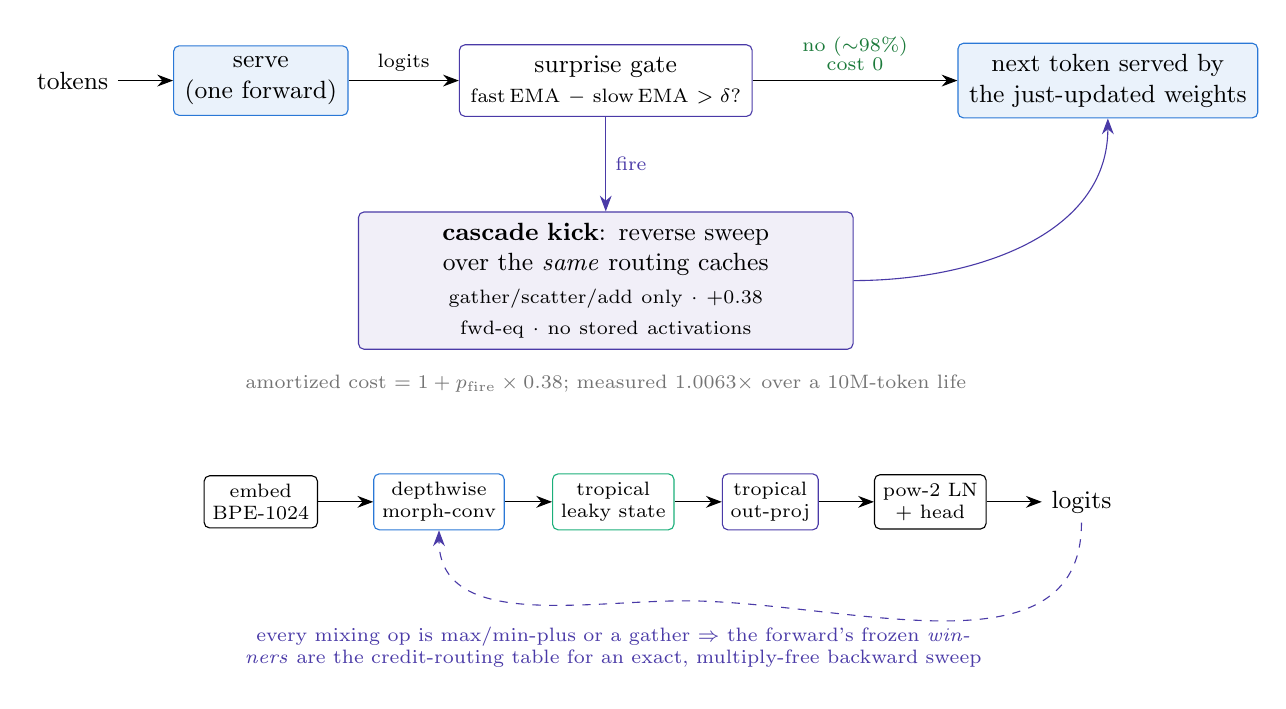
\begin{tikzpicture}[font=\small, >={Stealth[length=2mm]},
  box/.style={draw, rounded corners=2pt, inner sep=4pt, align=center},
  op/.style={draw, rounded corners=2pt, inner sep=3pt, align=center,
             font=\scriptsize}]
% --- top: the fused loop -----------------------------------------------
\node[box, fill=learner!10, draw=learner] (serve) {serve\\(one forward)};
\node[left=7mm of serve] (in) {tokens};
\node[box, right=14mm of serve, draw=firec] (gate) {surprise gate\\
   \scriptsize fast\,EMA $-$ slow\,EMA $>\delta$?};
\node[box, right=26mm of gate, draw=learner, fill=learner!10] (next)
   {next token served by\\the just-updated weights};
\node[box, below=12mm of gate, fill=firec!8, draw=firec, text width=6.0cm]
   (kick) {\textbf{cascade kick}: reverse sweep over the \emph{same} routing
   caches\\[1pt]\scriptsize gather/scatter/add only $\cdot$ $+0.38$ fwd-eq
   $\cdot$ no stored activations};
\draw[->] (in) -- (serve);
\draw[->] (serve) -- node[above,font=\scriptsize]{logits} (gate);
\draw[->] (gate) -- node[above,font=\scriptsize,text=goodc,align=center]
   {no ($\sim$98\%)\\[-1pt]cost 0} (next);
\draw[->,firec] (gate) -- node[right,font=\scriptsize]{fire} (kick);
\draw[->,firec] (kick.east) to[out=0,in=-90] (next.south);
\node[below=2mm of kick, font=\scriptsize, text=black!55]
   {amortized cost $=1 + p_{\mathrm{fire}}\times0.38$; measured $1.0063\times$
    over a 10M-token life};
% --- bottom: the substrate strip ---------------------------------------
\begin{scope}[yshift=-5.35cm]
\node[op] (emb) {embed\\ \scriptsize BPE-1024};
\node[op, right=7mm of emb, draw=learner] (conv) {depthwise\\morph-conv};
\node[op, right=6mm of conv, draw=normc] (state) {tropical\\leaky state};
\node[op, right=6mm of state, draw=firec] (proj) {tropical\\out-proj};
\node[op, right=7mm of proj] (head) {pow-2 LN\\+ head};
\node[right=7mm of head] (logit) {logits};
\foreach \a/\b in {emb/conv,conv/state,state/proj,proj/head,head/logit}
  \draw[->] (\a) -- (\b);
\draw[->,firec,dashed] (logit.south) to[out=-90,in=0]
   ($(conv.south)!0.5!(head.south)+(0,-0.9)$) to[out=180,in=-90] (conv.south);
\node[below=11mm of state, text width=11cm, align=center, font=\scriptsize,
      text=firec]
  {every mixing op is max/min-plus or a gather $\Rightarrow$ the forward's
   frozen \emph{winners} are the credit-routing table for an exact,
   multiply-free backward sweep};
\end{scope}
\end{tikzpicture}
\caption{\textbf{One process serves and learns.} Top: the fused loop. Every
token is served by one forward pass; a two-timescale surprise gate decides
per window whether that same pass also becomes a learning step. When it fires,
a \emph{cascade kick} routes output errors backward through the routing caches
the forward already produced---gather/scatter/add only, no second forward, no
stored activation graph---and steps the optimizer in place; the next token is
served by the updated weights. Bottom: the substrate, a tropical (max-plus)
MorphSSM language model in which every mixing operation is a maximum of sums or
a gather, so the winning paths cached during serving are exactly the table
needed to assign credit without multiplication.}
\label{fig:loop}
\end{figure*}

\heading{The fused step.}
The routine \texttt{serve\_and\_learn} runs one forward pass, returns the
logits (the serving product), evaluates the gate on the window's loss and---only
if the gate fires---runs the reverse sweep on the caches the forward already
produced, then steps the optimizer in place. There is no second forward, no
retained activation graph and no other process. Measured against serve-only,
the fused loop costs $1.23\times$ wall-clock time and $1.38\times$ operation
volume (a pre-fusion harness that re-ran the forward paid $2.23\times$/%
$2.38\times$); its peak learning memory is serve-class. Because the sweep never
materializes an activation graph, the same cascade trained a $d{=}832$ variant
in a memory budget where reverse-mode automatic differentiation exhausted
44~GB---a systems consequence of the substrate, not a tuning choice.

\heading{Credit assignment is exact, and stays exact at depth.}
The claim that one cascade sweep equals backpropagation is not asymptotic; it is
bitwise, and we test it directly (Fig.~\ref{fig:depth}a). Across 282 parameter
tensors spanning two architectures, three seeds and both the annealed and
deployed regimes, the cascade gradient has cosine similarity $1.000$ with the
backpropagation gradient and relative error at the $10^{-7}$ level (finite
floating-point summation order only); the cached-routing forward is bit-exact
with a standard forward. A synchronous reverse-topological relaxation reproduces
the cascade with zero difference, and asynchronous sweeps with only half the
layers participating per round still recover the exact gradient once messages
have propagated far enough---credit is either fully routed or not yet arrived,
never corrupted.

This exactness is what lets predictive coding work at depth where the naive
form fails. Iteratively settling the states of a deep predictive-coding network
is numerically unstable: the energy diverges and accuracy falls to chance even
at shallow depth. Our substrate instead relaxes the \emph{errors} with routing
frozen, which is triangular and therefore unconditionally stable, and collapses
to a single sweep. On a 128-layer residual network the multiplication-free
cascade trains to $0.94$ test accuracy while standard floating-point
backpropagation collapses to chance ($0.24$) and naive iterative predictive
coding never leaves chance (Fig.~\ref{fig:depth}b). On the sequence model used
throughout this paper, the cascade matches backpropagation's language-modelling
quality at every depth from 4 to 32 layers (Fig.~\ref{fig:depth}c). Depth, in
other words, is not bought at the price of the exactness or the
multiplication-free property (Supplementary Fig.~\ref{supp:depth}).

\begin{figure*}[t]
\centering
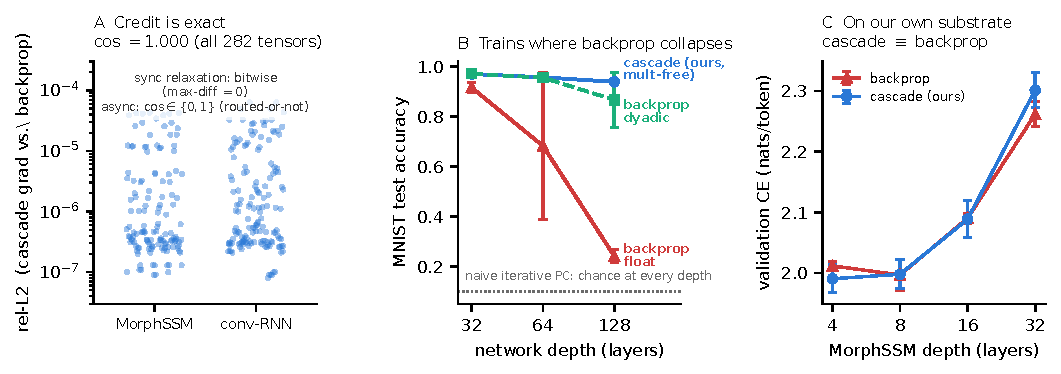
\includegraphics[width=\textwidth]{figs/fig_pcdepth.pdf}
\caption{\textbf{Predictive coding, made exact and deep by the substrate.}
\textbf{a}, The cascade update equals backpropagation's gradient: over all 282
parameter-tensor checks the cosine similarity is $1.000$ and the relative error
is $\sim\!10^{-7}$ (floating-point summation order); synchronous relaxation is
bitwise identical and asynchronous, partial-participation sweeps recover the
exact gradient (cosine $\in\{0,1\}$: routed or not-yet-arrived). \textbf{b}, On
a 128-layer residual network the multiplication-free cascade is the only method
that still trains; floating-point backpropagation collapses toward chance and
naive iterative predictive coding sits at chance for every depth (mean$\pm$s.d.,
three seeds). \textbf{c}, On our own tropical sequence model the cascade tracks
backpropagation's validation cross-entropy at every depth (mean$\pm$s.d., three
seeds). Data: \texttt{g0\_gradcheck}, \texttt{g1\_equivalence},
\texttt{scale\_mnist\_128layer}, \texttt{g3\_g4\_*}.}
\label{fig:depth}
\end{figure*}

\heading{The model and the streams.}
The learner is a MorphSSM language model: token embeddings pass through seven
layers of depthwise morphological (max-plus) convolution, a tropical leaky state
$h_t=\max(u_t,\,h_{t-1}-\lambda)$ with a learned non-negative leak (a
content-gated running maximum), and a tropical dilation/erosion output
projection; a power-of-two-scaled normalization and a linear head produce
logits. During pre-training the hard maximum is annealed from a soft
relaxation; all adaptation here runs in the deployed hard regime. The streams
are four text domains (encyclopedic text, Shakespeare, this project's
documentation, and its source code) presented as three non-stationary regimes
plus a stationary control. Throughout we use a prequential protocol: every
window is scored by the weights \emph{before} any learning from it; a frozen
twin is scored on identical windows; per-domain specialists trained to
convergence provide an oracle, and we report headroom captured, the fraction of
the frozen-to-oracle gap that the live learner closes.

\heading{Live learning pays.}
Across three short single-regime streams (hard-shift, drift, novel-vocabulary)
the gated learner's prequential regret against its frozen twin was $-2.97$,
$-2.92$ and $-1.58$ nats per token (three seeds, s.d.\ $\le0.023$), capturing
61--69\% of the frozen-to-oracle headroom at $1.13\times$ amortized serving cost
(the full rotated lifetime below captures $0.57$ at $1.006\times$; the shorter
two-cycle optimizer comparison, $0.41$--$0.62$; these are distinct protocols). On the
stationary control, learning bought nothing, exactly as it should: once the gate
is properly calibrated it essentially stops firing, and the small apparent
regret is a serving-mode artifact rather than update damage---an accounting trap
we flag for prequential comparisons generally.

\heading{A law of surprise gating.}
Always-on learning needs a rule for \emph{when} a served example also becomes an
update, and we find that this choice is not a tuning detail but obeys a law
(Fig.~\ref{fig:validation}b). A gate that fires when the window loss
exceeds its own running mean by a fixed number of running standard deviations
converges, on any stationary stream, to firing at a fixed tail quantile: it is a
rate limiter, not a novelty detector, because self-normalization erases exactly
the regime information the gate needs. Empirically such a gate fired at
indistinguishable rates on stationary and hard-shifted streams at every
threshold, and could never satisfy the natural calibration criterion, ``be quiet
when there is nothing to learn.'' The constructive fix removes the
normalization: fire when a fast exponential moving average of the loss exceeds a
slow one by an absolute margin in nats. On stationary data both timescales
converge and the gap vanishes, so the gate self-quiets by construction (fire
rate $0.01$--$0.24\%$ versus $27$--$36\%$ for the self-normalized family); a
distribution shift opens the gap by the loss jump itself. This margin gate
retains 90\% of the adaptation benefit at a third of the updates. We suggest
that deployed surprise gates should be tested against the self-quieting
criterion.

\heading{An honest comparison to the deployed incumbent.}
The standard way to keep a deployed model current is to buffer the stream and
periodically fine-tune low-rank adapters (LoRA) with a few gradient
steps\cite{hu2022lora}. We built this incumbent to win: a dense transformer,
warm-started to \emph{exactly} our checkpoint's pre-training quality and served
in evaluation mode, with rank, cadence and learning rate swept and a
drift-triggered schedule included, plus full fine-tuning and per-window online
backpropagation as anchors. On identical streams (Fig.~\ref{fig:validation}) no
incumbent configuration lies below-and-left of ours: the cheapest cell that
beats our quality pays $3.3\times$ our update compute and sits in a
$2.7\times$ larger activation-memory class (138 versus 51~MB), and the
low-compute frontier is ours. Graphics processors keep the
unconstrained-compute end, exactly the pre-registered segmentation. Two honest
notes travel with this result. The dense model reached the shared warm-start
quality in 1{,}150 optimizer steps against our substrate's 8{,}699 (a real
capability ceiling; see below), and the incumbent's always-on
online-backpropagation arm \emph{hurts} on stationary data---unconditional
updating damages any substrate, so gating is a universal requirement, not a
patch for ours.

\begin{figure}[t]
\centering
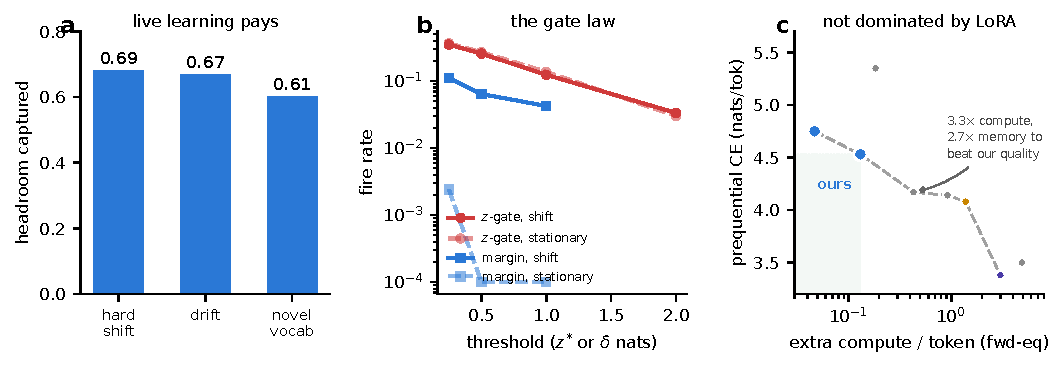
\includegraphics[width=\textwidth]{figs/fig_validation.pdf}
\caption{\textbf{The loop pays, self-calibrates, and is not dominated.}
\textbf{a}, Headroom captured on three short single-regime streams (gated learner,
mean over three seeds). \textbf{b}, The gate law: a self-normalized $z$-gate fires
at a fixed quantile regardless of regime (stationary and shifted indistinguishable),
while the two-timescale absolute-margin gate self-quiets on stationary data and
storms at shifts. \textbf{c}, Quality versus extra update compute on identical
streams: our two operating points hold the low-compute frontier; no incumbent cell
lies below-and-left of ours, and matching our quality costs a tuned LoRA-periodic
incumbent $3.3\times$ our update budget and a $2.7\times$ activation-memory class
(single seed on the incumbent sweep; our side three-seed). Data: \texttt{v2\_live},
\texttt{v3\_lora}.}
\label{fig:validation}
\end{figure}

\heading{A device life.}
To test retention we ran a single process over ten million served tokens in five
rotated cycles of the four domains (Fig.~\ref{fig:lifelong}). The live learner
tracked the moving stream while its frozen twin re-paid the full cost of every
shift forever. Headroom captured was $0.57\pm0.03$ over three seeds at
$1.0063\times$ serving cost: the gate fired on 1.65\% of windows over the whole
life, collapsing from 1{,}275 kicks in the first cycle to 45 in the fifth, with
two late eras fully silent---the device learned its world, then mostly just
served. Retention is a stability--plasticity trade, reported as such: the
encyclopedic-specialist birth model gave up some of its specialty for a
generalist basin that was on average far better across domains, and held it with
bounded, non-increasing interference across cycles (Fig.~\ref{fig:lifelong}c,d). The weight norm reached equilibrium (a $2.3\%$ rise
over the life, its slope decelerating twelvefold), a dedicated adversary
survived 20{,}833 consecutive updates---$3.5\times$ the horizon at which our
strict-optimizer runs historically collapsed---and a 5\% sampled audit of
1{,}236 kicks across four lives found zero multiplications; the entire update
stream is replayable from the seed and checkpoint chain.

\begin{figure}[t]
\centering
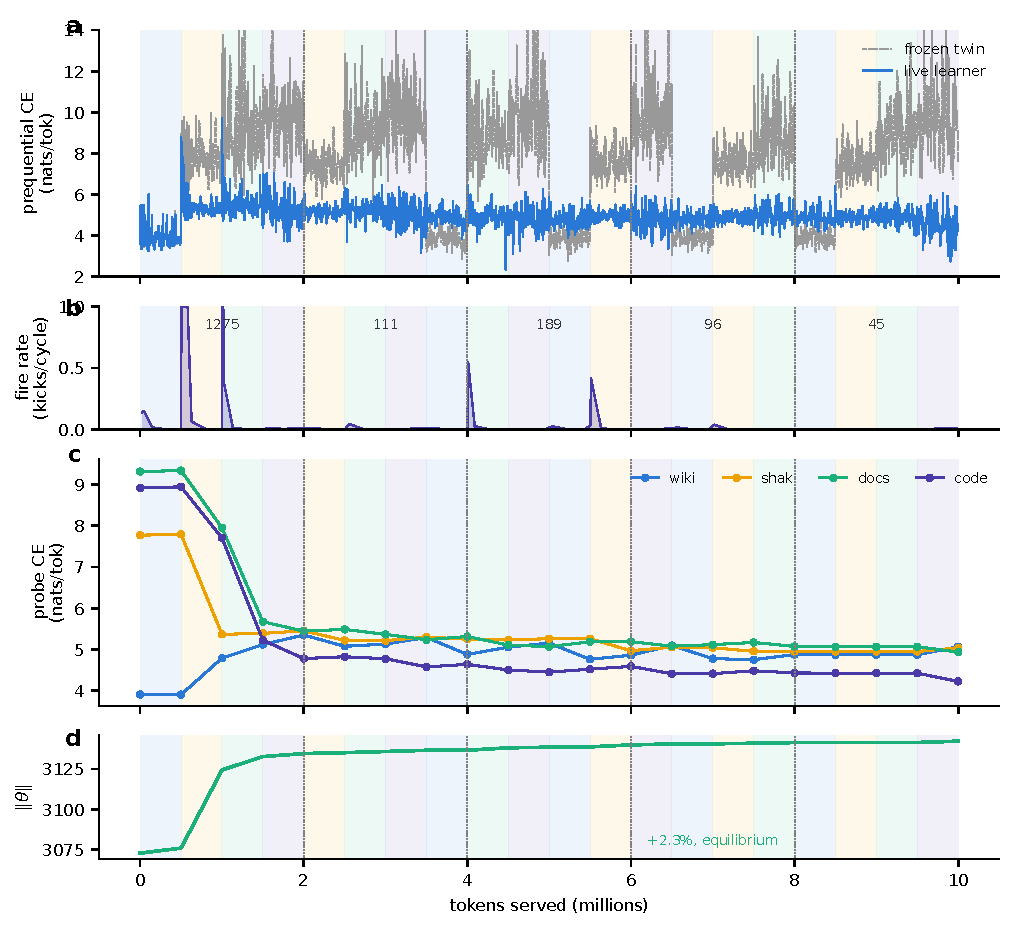
\includegraphics[width=\columnwidth]{figs/fig_lifelong.pdf}
\caption{\textbf{A lifelong stream of experience: one process, ten million tokens,
five rotated domain cycles.} \textbf{a}, Prequential cross-entropy of the live
learner (blue) versus its frozen twin (grey); shaded bands mark domains, dotted
lines mark cycles. The learner storms down at each first encounter, then serves
revisits almost for free, while the frozen twin re-pays the full cost forever.
\textbf{b}, Gate fire rate; learning kicks collapse from 1{,}275 to 45 per cycle.
\textbf{c}, Held-out probe cross-entropy per domain at every era boundary---after
the first cycle the stability--plasticity trade is stable and improves with
revisits (bounded, non-increasing interference). \textbf{d}, Weight norm reaches
equilibrium ($+2.3\%$ over the life; slope decelerates twelvefold). Data:
\texttt{v4\_tele\_main}, \texttt{v4\_probes\_main}.}
\label{fig:lifelong}
\end{figure}

\heading{Silicon energy is below the floor.}
The substrate's training kernels run on Amazon Web Services F2 FPGAs with the
digital-signal-processing multipliers verifiably absent and known-answer tests
matching host references bitwise; a trainer converged on-fabric during the
measurement windows on a trajectory equal to simulation. The energy question was
pre-registered with an honest-negative branch, which is what we report: on the
core-rail telemetry (quantized at one watt) idle, serving and serving-while-%
learning all sit at 4.0--4.6~W, so the marginal power of learning is below the
instrument's resolution ($\le1$~W on a $\sim$4~W rail), and at the life's fire
rate its amortized addition is unmeasurable. The comparison that survives the
core-rail-versus-board-power caveat is regime-level: a contemporary graphics
processor drew a measured 79~W of board power \emph{merely serving} the same
single-example stream. Board-level and application-specific-integrated-circuit
figures await external instrumentation and are not claimed here. Even as a
bound, the direction is unambiguous, and taken together with the low-compute
frontier of Fig.~\ref{fig:validation}c and the fully replayable audit trail it
points at an operating regime today's practice does not occupy: a model that
keeps adapting \emph{where it runs}---at the sensor, in the field, on data that
never leaves the device---with no training cluster, no second memory system, and
no power budget for learning that the instrument can even resolve.

\heading{From perception to agency.}
The framing we find most consequential is not language modelling but agency---the
prospect of agents that inhabit \emph{streams of experience} and learn continually
over a lifetime, rather than from short, curated episodes\cite{silver2025experience}.
Yet in deployed reinforcement-learning systems, ``online'' learning still
instantiates the acting policy and the learning process as different programs,
often on different machines, coupled by replay buffers and parameter
servers\cite{espeholt2018impala,horgan2018distributed,sutton1991dyna}; even
single-process streaming agents alternate environment steps with gradient steps
that traverse a distinct backward graph\cite{elsayed2024streaming}. In every
case the agent \emph{stops being only an actor} in order to learn. The loop
validated here dissolves that boundary for supervised prediction: the forward
pass that produces behaviour is, unchanged, the sufficient statistic for the
weight update, and the next act is taken by the just-updated weights. This is the
difference between an agent that \emph{has} a training pipeline and an agent
whose \emph{experience is its training}---closer to the always-plastic character
of biological learning than to the train-then-deploy dichotomy (Box~1;
Supplementary Figs.~\ref{supp:org} and~\ref{supp:neuro}). What the
loop does not yet provide is the reinforcement-learning problem itself---credit
over actions and delayed reward; here surprise is the only teacher. Extending the
fused loop from prediction to control, without reintroducing the actor/learner
split, is in our view the right next problem.

% ---------------------------------------------------------------------
% BOX 1 : the neuroscience map
% ---------------------------------------------------------------------
\begin{figure}[t]
\centering
\fbox{\begin{minipage}{0.94\columnwidth}
\small
\textbf{Box 1\,$\vert$\, A cortical reading of the loop (a source of hypotheses,
not a claim of biological fidelity).}\\[3pt]
The design rhymes with several principles from systems neuroscience. We list the
correspondences because they generated the design and suggest tests, not because
the analogy proves anything; every claim in this paper is settled by the
measurements, not by the mapping.
\vspace{3pt}
\begin{tabular}{@{}p{0.30\linewidth}p{0.63\linewidth}@{}}
\toprule
\textbf{neuroscience} & \textbf{this loop} \\
\midrule
predictive coding in cortex\cite{rao1999predictive} & the substrate settles
prediction errors; the cascade is the exact fixed point\cite{song2020can} \\
no weight transport (the classic objection to backprop)\cite{lillicrap2020backpropagation,lillicrap2016random}
& credit flows through the forward's own routing caches; neighbour-only
messages, no separate backward weights \\
neuromodulated, error-gated plasticity (three-factor rules)\cite{fremaux2016neuromodulated}
& the surprise gate is a global ``learn now'' signal, not a gradient path \\
perceptual priors and their precision resolve ambiguity\cite{friston2010free,flounders2019neural}
& consolidated weights are the slow prior; a fired update's \emph{precision}, not
its magnitude, sets what is protected \\
ongoing activity is not idle; prediction is continuous\cite{keller2018predictive,flounders2019neural}
& the device is always on its stream---serving is the ongoing prediction, learning
an occasional gated consequence of it \\
complementary learning systems; consolidation\cite{mcclelland1995complementary,kumaran2016learning,benna2016computational}
& fast in-place kicks plus a slow precision anchor toward a weight posterior \\
metabolic efficiency ($\sim$20~W)\cite{attwell2001energy} & learning is
energetically invisible against serving on the measured substrate \\
\bottomrule
\end{tabular}
\vspace{2pt}\\
\footnotesize These links are deliberately falsifiable: the self-quieting gate
predicts that a useful neuromodulatory surprise signal must decorrelate from
stimulus variance; the routing-cache mechanism predicts that exact credit needs no
symmetric feedback weights\cite{lillicrap2016random,payeur2021burst,
bellec2020solution}; and the anchor predicts that what a synapse consolidates is
set by the precision of its predictions, not by how much it has recently moved.
\end{minipage}}
\label{box:neuro}
\end{figure}

\heading{What the evidence supports, and what it does not.}
A single process can serve and learn at about $1.4\times$ a forward pass per
fired update and about $1.006\times$ amortized over a realistic life, exactly
implementing gradient descent, with no multiplications in the serve-and-learn
sweep and no activation memory, on hardware where the learning is energetically
negligible. The reverse sweep is multiply-free at every gate; the flagship life
additionally runs an AdamW optimizer (a declared audit boundary), and a fully
closed optimizer makes the whole loop multiply-free at a stated headroom cost
(Extended Data Table~\ref{tab:opt}). The claim is architectural, not statistical: nothing here says this
learner is more sample-efficient than backpropagation---it \emph{is}
backpropagation, on a substrate and schedule that make it fusible into serving.
The limitations are equally concrete and are the agenda for scaling this result
(Methods, ``Limitations and outlook''): the substrate has a genuine capability
ceiling (a dense transformer reaches matched pre-training quality in roughly
sevenfold fewer steps and generalizes better when frozen); all results are at a
small scale ($\sim$1M parameters), and our larger silicon runs surfaced an
unresolved backward-path divergence that gates scaling; the FPGA measurement
bounds core power only; and two pre-registered negatives---Fisher-weighted fleet
merging fails under sparse gated firing, and the capability ceiling above---are
part of the record. We report them because the value of this work is precisely
that the fused, audited, lifelong loop holds up when its parts are measured
honestly. The broader implication follows once acting and learning need not be
separate systems: continual, auditable, low-power adaptation becomes a property
of serving itself rather than a pipeline attached to it---a design space nearer
to how biological systems learn, and one that opens wherever a model must keep
pace with a world that does not pause for a training run.

% ======================================================================
% METHODS
% ======================================================================
\vspace{6pt}
\section*{Methods}
\small

\heading{Substrate and the cascade equivalence.}
The learner is a seven-layer MorphSSM ($d{=}256$, BPE-1024 tokenizer,
$\sim$1.0M parameters). Writing the network as a feedforward directed acyclic
graph of tropical operations, a predictive-coding relaxation with the standard
chain-rule loss admits a closed-form fixed point; substituting it layer by layer
yields a single reverse sweep (the cascade) whose parameter updates equal the
settled iterative predictive-coding updates and equal backpropagation's
gradients. Because weights enter additively through winning paths, at hard
routing each gradient entry is a signed count-weighted sum of output errors
routed through cached argmax indices, so the sweep contains no multiplications.
We enforce this with a dispatch-level auditor whose waivers are declared:
batch-mean divides, the lookup-table exponential and, in the research arm used
for the incumbent comparison and the life, the AdamW/anchor optimizer arithmetic,
recorded per step. The fully closed configuration (lookup-table loss plus a
sign-and-shift optimizer, \texttt{PureTropicalSGD}, characterized below) audits
clean end to end. The equivalence is the Z-IL
lineage\cite{song2020can}, not a new theorem; we contribute its bitwise
verification on every architecture used here, including under asynchronous,
partial-participation sweeps (Fig.~\ref{fig:depth}a).

\heading{A fully closed optimizer (retiring the AdamW waiver).}
The optimizer waiver above is not essential; the loop also runs with no waiver at
all. On a gated drift life (a shorter two-cycle variant of the lifetime protocol,
single seed) we compare multiply-free optimizers against AdamW (Extended Data
Table~\ref{tab:opt}). A sign-based, bounded leaky-integer update
(\texttt{PureTropicalSGD})---biologically shaped as potentiation/depression on a
low-precision synaptic state\cite{bartol2015nanoconnectomic}, audited to contain
zero multiplications---captures $0.41$ of the frozen-to-oracle headroom,
two-thirds ($67\%$) of anchorless AdamW's $0.62$ (and $79\%$ of AdamW's anchored
operating point, $0.52$, which itself trades plasticity for retention), with no
collapse. An error-feedback
variant additionally cures a consecutive-update adversary that the naive sign rule
does not survive (regret $+0.90\!\to\!-0.01$; the soft-bound alone does not;
Extended Data Fig.~\ref{fig:efabl}), but error feedback's conservatism costs
plasticity ($0.07$), so no single closed optimizer is at once maximally plastic and
adversary-immune. The residual gap to AdamW is per-parameter variance
normalization, which multiply-free sign updates do not replicate at this
scale---a quantified limitation. With \texttt{PureTropicalSGD} the serve-and-learn
loop is multiply-free \emph{and} Adam-free end to end at a stated quality cost;
closing the gap (a closed variance normalization for plasticity, and precision-%
derived consolidation for retention) is future work.

\heading{Depth experiments.}
Figure~\ref{fig:depth}b uses residual multilayer networks on MNIST (hidden 256,
eight epochs, three seeds) comparing the cascade, dyadic backpropagation and
floating-point backpropagation at depths 32/64/128, plus a naive
iterative-settling arm that diverges to chance at every depth. Panel c uses the
paper's MorphSSM language model at depths 4/8/16/32 (three seeds), reporting
final hard-routing validation cross-entropy. Panel a aggregates 282 parameter
tensors from gradient-check runs (two architectures, $\tau\in\{0.5,0\}$, three
seeds) and the synchronous/asynchronous relaxation equivalence runs. On plain
(non-residual) deep networks all methods, including floating-point
backpropagation, collapse with depth; the tropical max-residual is what makes
depth trainable, and we report the residual configuration accordingly.

\heading{The fused step and cost.}
\texttt{serve\_and\_learn} serves with one forward, evaluates the gate on the
window loss and, on firing, runs the reverse sweep on the serving forward's
caches and steps the optimizer in place. Cost multipliers are measured by an
operation-count tracer and wall-clock timing against a serve-only baseline; the
op-volume figure is deterministic. Peak memory is measured for serve,
serve+cascade and serve+backpropagation. The $d{=}832$ out-of-memory comparison
used identical model, data and 44~GB budget; the cascade trained while
reverse-mode autograd exhausted memory.

\heading{Streams, protocol and metrics.}
Four public/self text domains (0.8--5~MB) are tokenized at BPE-1024; the learner
is warm-started from a text8-trained checkpoint. Regimes are hard-shift, drift,
novel-vocabulary and a stationary control. The protocol is prequential (score
before learn); a frozen twin is scored on identical windows; per-domain oracles
(converged specialists) give the headroom denominator. Headroom captured is
$1-R_{\mathrm{oracle}}/R^{\mathrm{frozen}}_{\mathrm{oracle}}$. We report regret
versus the frozen twin, headroom captured, amortized cost, adaptation latency,
weight-norm trajectory, a forgetting transfer matrix and audit coverage, always
with the per-token cost histogram rather than a bare mean.

\heading{The gate.}
The self-normalized gate fires when window loss exceeds a running mean by
$z^{*}$ running standard deviations; we show analytically and empirically that
its stationary fire rate is the fixed quantile $P(z>z^{*})$, independent of
regime. The margin gate fires when a fast EMA (coefficient 0.9) of the loss
exceeds a slow EMA (0.999) by an absolute margin $\delta$ nats; the life uses
$\delta{=}0.25$. Both cost one scalar per window.

\heading{Incumbent comparison.}
The incumbent buffers the stream and periodically runs $K$ AdamW steps on LoRA
adapters (rank $\times$ cadence $\times$ learning rate swept; drift-triggered
cadence, full fine-tuning and per-window online backpropagation included), from a
dense transformer warm-started to our checkpoint's pre-training quality within a
two-sided tolerance and served in evaluation mode. The budget currency is extra
update compute per served token in forward-equivalents of each method's own
serving cost; the activation-memory class is measured separately. The incumbent
sweep is single-seed; our side is three-seed.

\heading{The life.}
The organism configuration (margin gate $\delta{=}0.25$; precision anchor
$\lambda{=}0.01$ on the optimizer's own second moments; learning-rate halving on
a fired-kick schedule; serving dropout off) ran 104{,}160 windows in one process
as a daemon with kill-safe bit-exact resume, an append-only ledger and
clone-isolated probes. Retention probes are fixed held-out sets, never streamed.
The adversary rider ran 20{,}833 consecutive updates with the gate bypassed. The
audit sampled 5\% of kicks; optimizer arithmetic lies outside the audited region
(a declared boundary).

\heading{Silicon.}
Kernels run on AWS F2 FPGAs; multiplier absence and known-answer parity are
checked on fabric. Core-rail (Vccint) power telemetry quantizes at one watt.
The GPU board-power contrast (A10G, \texttt{nvidia-smi}) uses identical streams
and tokens. Board-level parity is explicitly not claimed; the FPGA figure feeds
an application-specific-integrated-circuit study as a floor input.

\heading{Relation to prior work.}
Tropical/max-plus and multiplication-free networks\cite{zhang2018tropical,
zhu2024matmulfree,tropicalattention2025,morpmamba2024}; predictive-coding/%
backpropagation equivalence\cite{rao1999predictive,millidge2022predictive,
whittington2017approximation,song2020can}; continual learning and loss of
plasticity\cite{kirkpatrick2017overcoming,dohare2024loss}; test-time and
streaming adaptation\cite{sun2020test,elsayed2024streaming}; efficient
fine-tuning\cite{hu2022lora}; and biologically motivated local learning
rules\cite{lillicrap2016random,fremaux2016neuromodulated,bellec2020solution,
payeur2021burst}. We use these substrates and rules; the fused, audited,
lifelong loop is the contribution.

\heading{Limitations and outlook.}
(i) \emph{Capability ceiling}: at matched pre-training quality a dense
transformer trains in about sevenfold fewer steps and generalizes better when
frozen; our substrate currently wins only the always-on, low-power segment.
(ii) \emph{Scale}: results are at $\sim$1M parameters; a 30M-parameter silicon
run surfaced an unresolved backward-path divergence that gates scaling.
(iii) \emph{Board power}: the FPGA rail bounds core power only. (iv) The margin
gate is blind to entries into intrinsically easier domains; difficulty-%
normalized (excess-surprise) gating is unfinished. (v) The incumbent sweep is
single-seed. (vi) \emph{Closed-optimizer gap}: the fully multiply-free optimizer
captures $67$--$79\%$ of AdamW's headroom (Extended Data Table~\ref{tab:opt}); the
residual gap is per-parameter variance normalization, which sign-based updates do
not replicate. The near-term agenda is a closed variance normalization and
precision-derived consolidation to close that gap, difficulty-normalized gating,
resolving the scale-blocking backward divergence, and extending the fused loop from
prediction to action-conditional control.

\heading{Data availability.}
All manuscript numbers derive from committed result logs (JSON-lines) under
\texttt{results/} (the substrate: \texttt{pc\_convrnn/}, \texttt{predictive\_%
coding/}) and \texttt{ontogenic\_learner/results/st\_stream/} (the loop and the
life). The four stream domains are public corpora (text8-derived encyclopedic
text, Shakespeare) and this project's own documentation and source code; no
other human data was used.

\heading{Code availability.}
The substrate, the fused \texttt{serve\_and\_learn} loop, the gate, the
closed optimizers (\texttt{PureTropicalSGD}, \texttt{EFTropicalSGD}) and the
precision anchor, the zero-multiply auditor, and the figure-generating scripts
(\texttt{make\_figs.py}, \texttt{make\_figs\_nature.py},
\texttt{make\_fig\_efablation.py}, \texttt{make\_fig\_optimizer.py}) are part of
the project repository; every figure regenerates from the committed logs.

% ======================================================================
% EXTENDED DATA
% ======================================================================
\clearpage
\section*{Extended Data}
\small
\setcounter{figure}{0}
\setcounter{table}{0}
\captionsetup[figure]{name=Extended Data Fig.}
\captionsetup[table]{name=Extended Data Table}
\vspace{6pt}

\begin{table}[h!]
\centering
\caption{\textbf{The pre-registered validation ladder.} Every gate's pass/kill
criteria were fixed before its run.}
\begin{tabular}{@{}lp{0.72\linewidth}@{}}
\toprule
gate & verdict \\
\midrule
V0 & \textbf{pass}: fused loop $1.23\times$ wall / $1.38\times$ ops; gradients
bitwise $\equiv$ backprop; zero-multiply audit clean \\
V1 & \textbf{pass}: streams admissible (per-domain headroom 6.7--10 bits/token;
stationary control 0.08); tokenizer identity exact \\
V2 & \textbf{pass}: regret $-1.6$ to $-3.0$ nats/token vs.\ frozen; headroom
captured 0.61--0.69 at $1.13\times$ serve (3 seeds) \\
V2b & \textbf{law}: self-normalized gates cannot self-quiet (fixed-quantile);
absolute-margin gate replaces them \\
V3 & \textbf{pass}: frontier held vs.\ tuned LoRA-periodic incumbent
(Fig.~\ref{fig:validation}) \\
V4 & \textbf{pass}: the 10M-token life; all retention criteria (headroom
$0.57\pm0.03$, norm equilibrium, non-increasing interference, 0/1{,}236 audit) \\
V4b & \textbf{negative}: Fisher merge loses to naive averaging under sparse gated
firing \\
V5 & \textbf{floor}: learning adds $\le1$~W to a $\sim$4~W rail; GPU serves the
same stream at 79~W board \\
\bottomrule
\end{tabular}
\label{tab:ladder}
\end{table}

\begin{table}[t]
\centering
\caption{\textbf{Multiply-free optimizers vs.\ AdamW} on the gated drift life
(headroom captured; single seed) and under a consecutive-update adversary. No
closed arm reaches AdamW's plasticity, and no single closed arm is both maximally
plastic and adversary-immune; \texttt{PureTropicalSGD} is the closed default (gate
provides stability), error feedback is adversary insurance. Data:
\texttt{v4\_life}, \texttt{v4\_tele\_precut\_*}.}
\begin{tabular}{@{}lccc@{}}
\toprule
optimizer & multiply-free & headroom & adversary \\
\midrule
AdamW (anchored) & no (4 ops) & 0.52 & --- \\
AdamW (anchorless) & no & 0.62 & --- \\
\texttt{PureTropicalSGD} & \textbf{yes} & \textbf{0.41} & collapses \\
\texttt{EFTropicalSGD} & \textbf{yes} & 0.07 & \textbf{survives} \\
\ \ +\,adaptive step & \textbf{yes} & 0.06 & survives \\
\bottomrule
\end{tabular}
\label{tab:opt}
\end{table}

\begin{figure}[t]
\centering
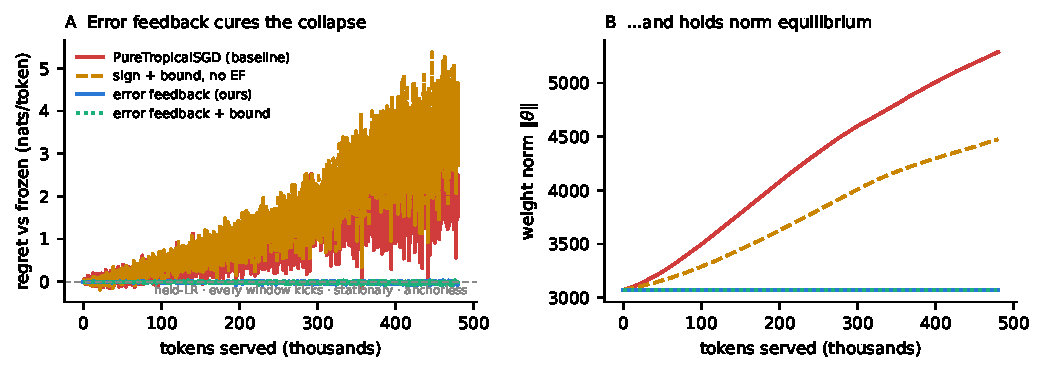
\includegraphics[width=\columnwidth]{figs/fig_efablation.pdf}
\caption{\textbf{Error feedback cures the sign-SGD collapse.} On a held-LR,
every-window-kicks, stationary, anchorless adversary, naked \texttt{PureTropicalSGD}
and a soft-bound-only variant diverge (regret climbs, weight norm runs away) while
the error-feedback arms stay flat at zero regret and constant norm --- the
$2{\times}2$ ablation attributes the cure to error feedback, not the soft-bound.
Fully multiply-free. Data: \texttt{v4\_tele\_precut\_*}.}
\label{fig:efabl}
\end{figure}

% ======================================================================
% SUPPLEMENTARY INFORMATION  (conceptual overviews)
% ======================================================================
\clearpage
\section*{Supplementary Information}
\small
\setcounter{figure}{0}
\captionsetup[figure]{name=Supplementary Fig.}

\begin{figure}[h!]
\centering
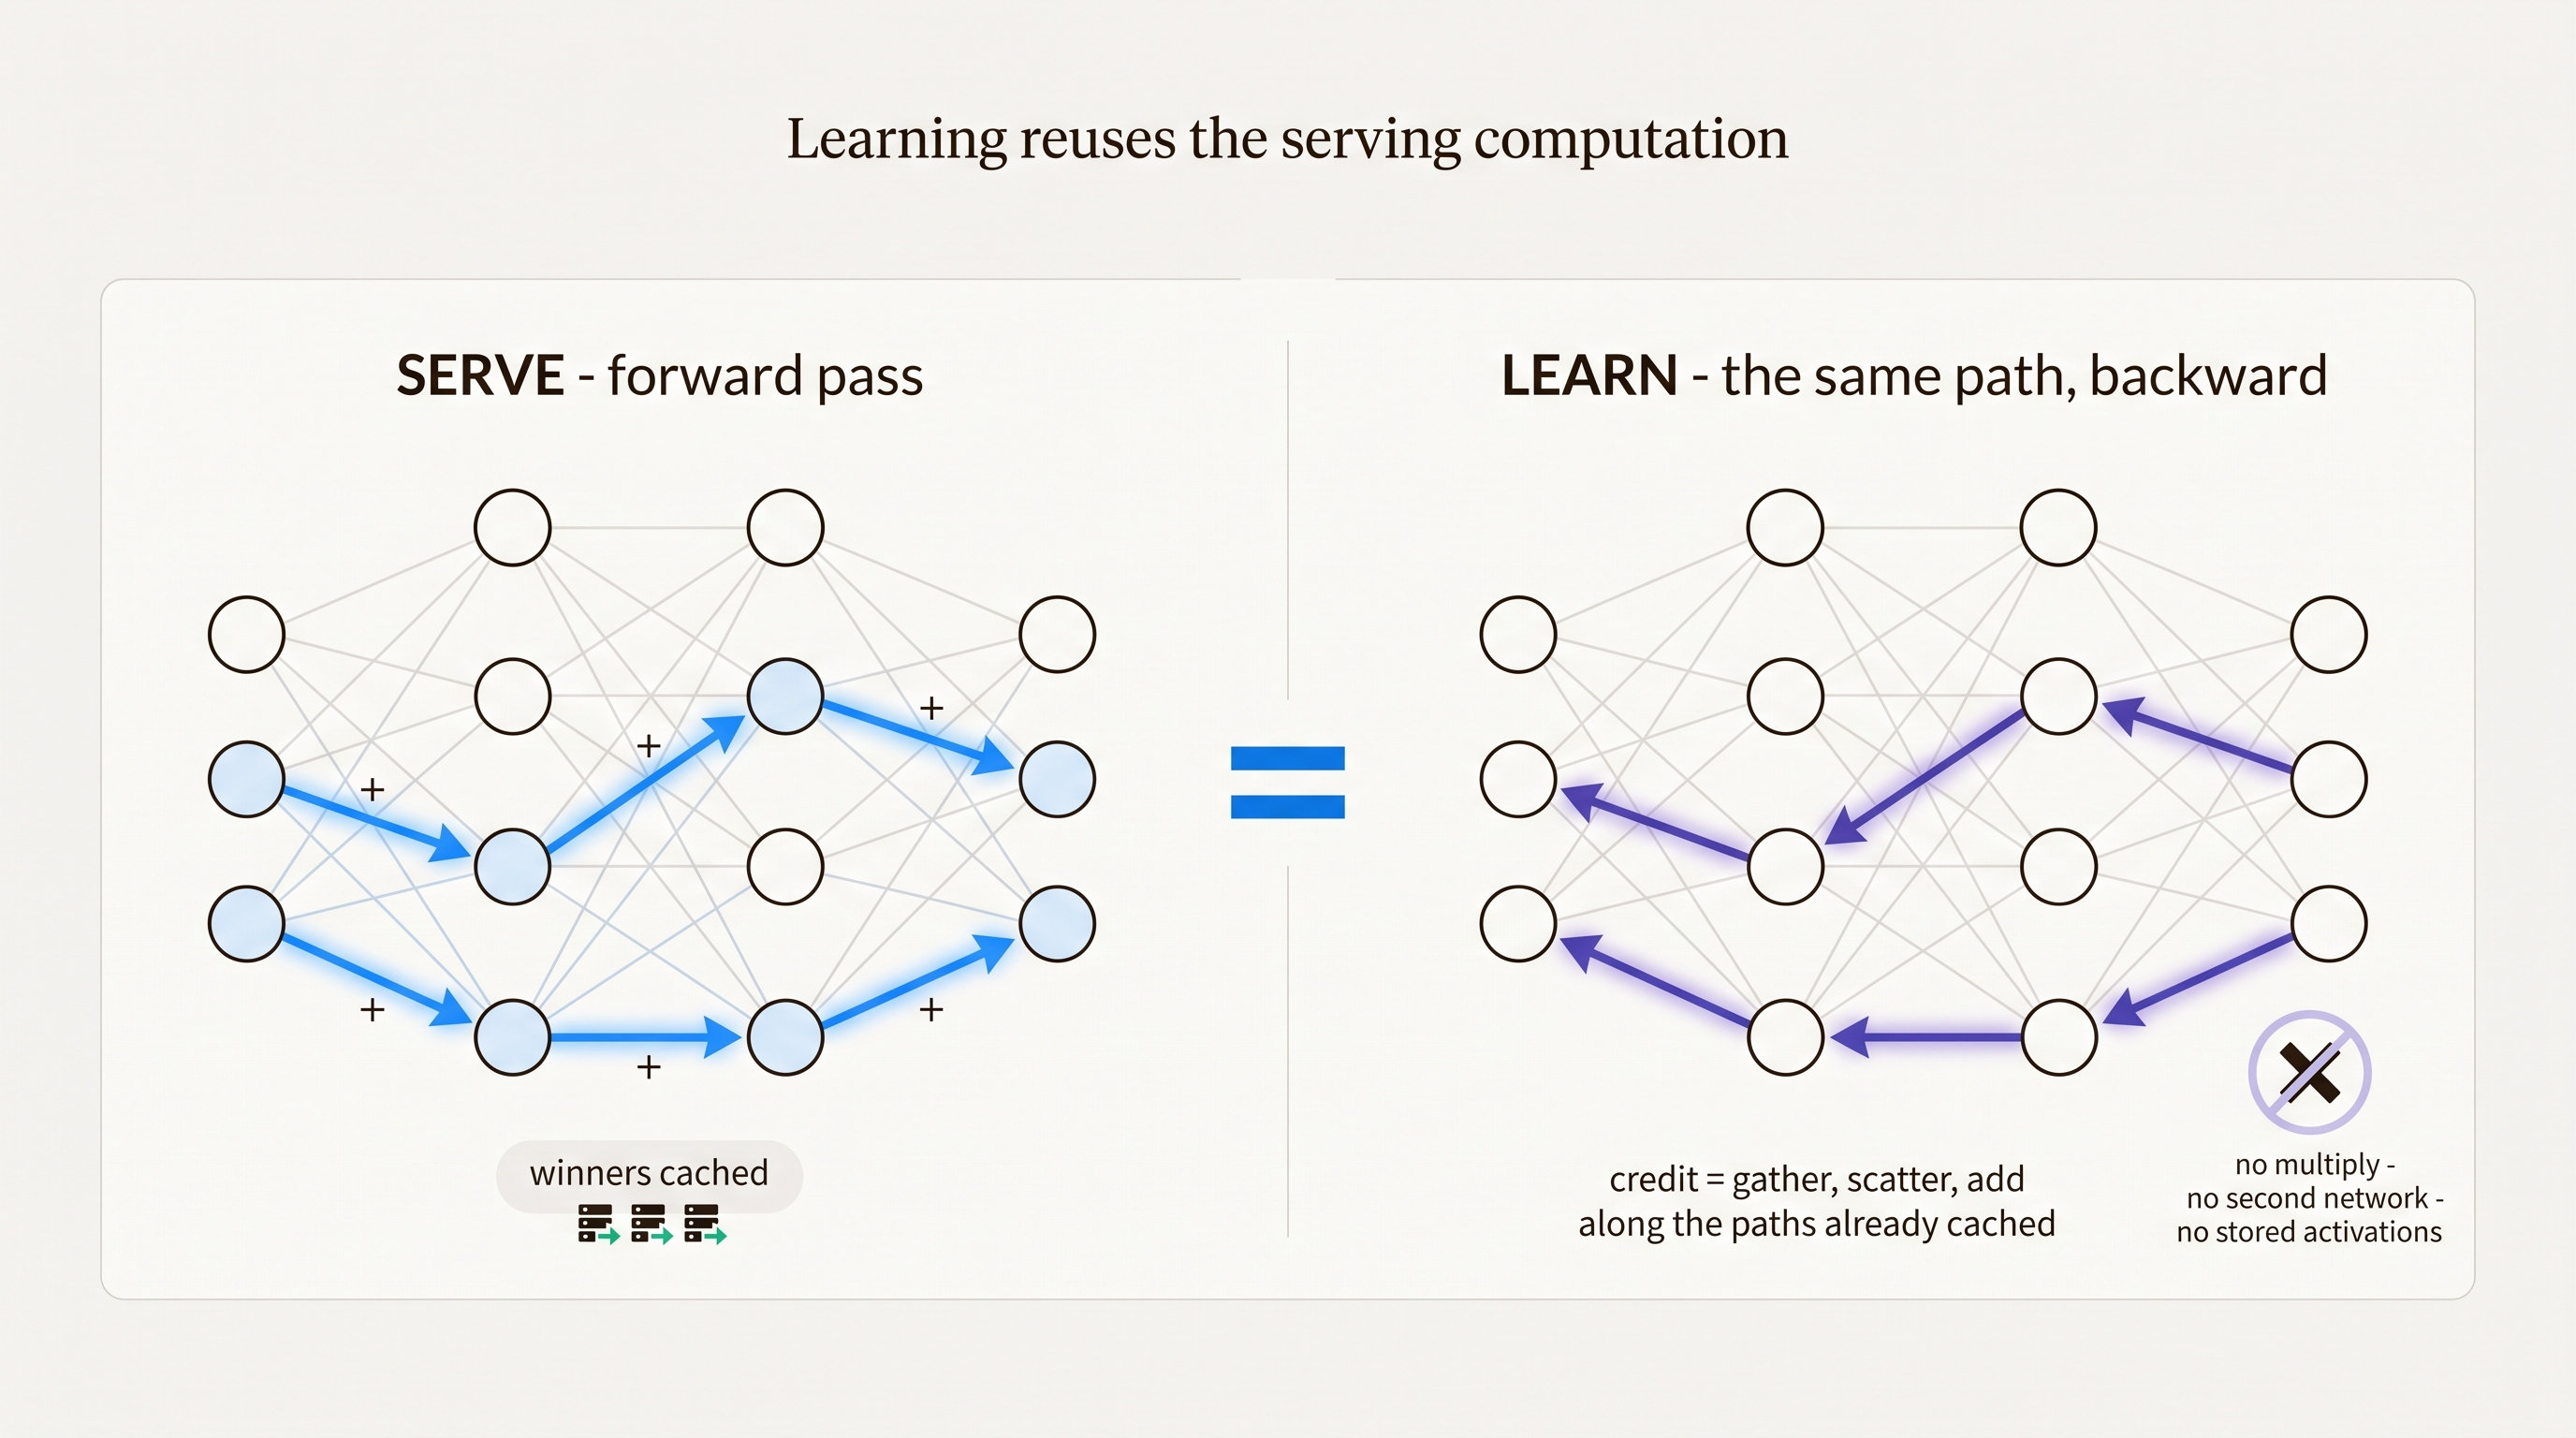
\includegraphics[width=\textwidth]{figs/gen/supp_pc.jpg}
\caption{\textbf{Why the tropical substrate makes learning free of a second
computation.} Serving runs the forward pass of a max-plus (tropical) network:
in each layer a single winning path is selected and its winners are cached
(left, blue). Learning is the \emph{same} cached path traversed backward
(right, purple): assigning credit is a gather/scatter/add along routes the
forward pass already committed---no multiplication, no second network, and no
stored activation graph. This is the visual statement of the mechanism in
Fig.~\ref{fig:loop} and the exactness measured in Fig.~\ref{fig:depth}a.
Conceptual illustration.}
\label{supp:pc}
\end{figure}

\begin{figure}[h!]
\centering
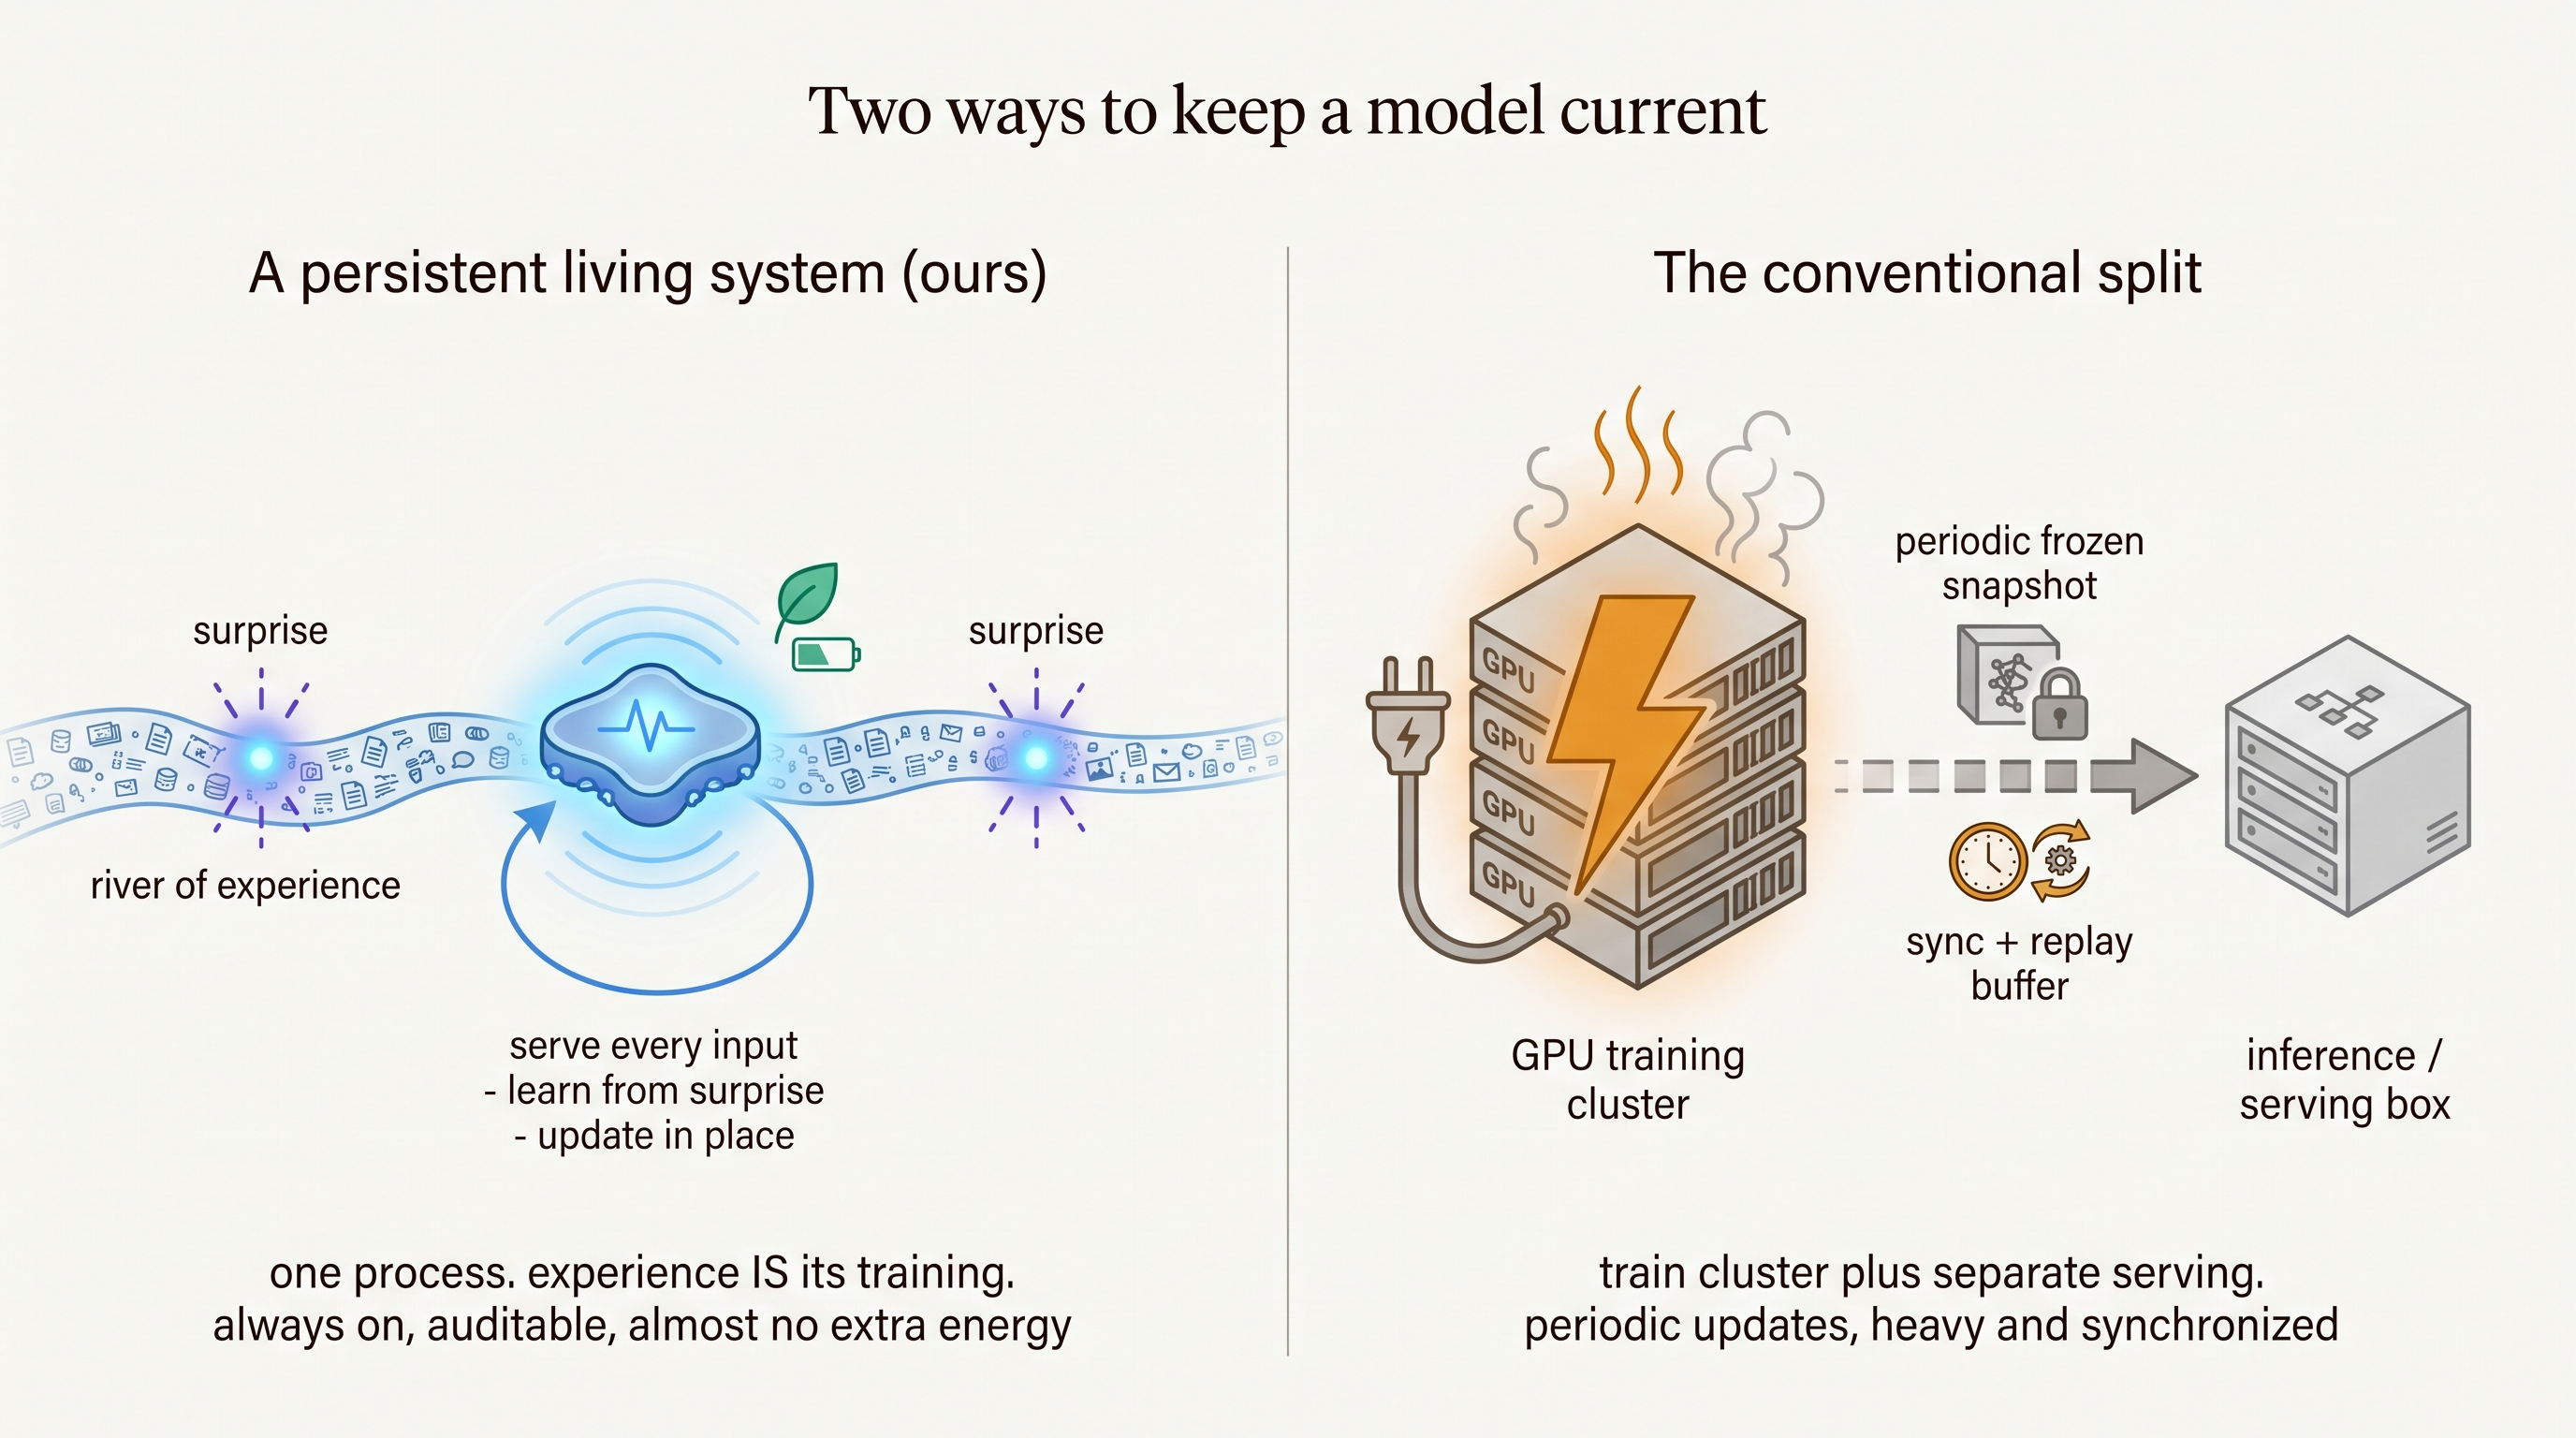
\includegraphics[width=\textwidth]{figs/gen/supp_organism.jpg}
\caption{\textbf{A persistent living system versus the conventional split.}
Left: our loop is one always-on process sitting on its stream of experience,
serving every input and---when surprised---learning in place, at energy so low
it is below the measurement floor; the experience \emph{is} the training, and
every update is auditable. Right: the deployed norm keeps a model current with a
separate, power-hungry training cluster that periodically ships a frozen
snapshot to a distinct serving system, coupled by synchronization and replay
storage. The paper's contribution is collapsing the right-hand picture into the
left one for supervised prediction (main text, ``From perception to agency'';
Box~1). Conceptual illustration.}
\label{supp:org}
\end{figure}

\begin{figure}[h!]
\centering
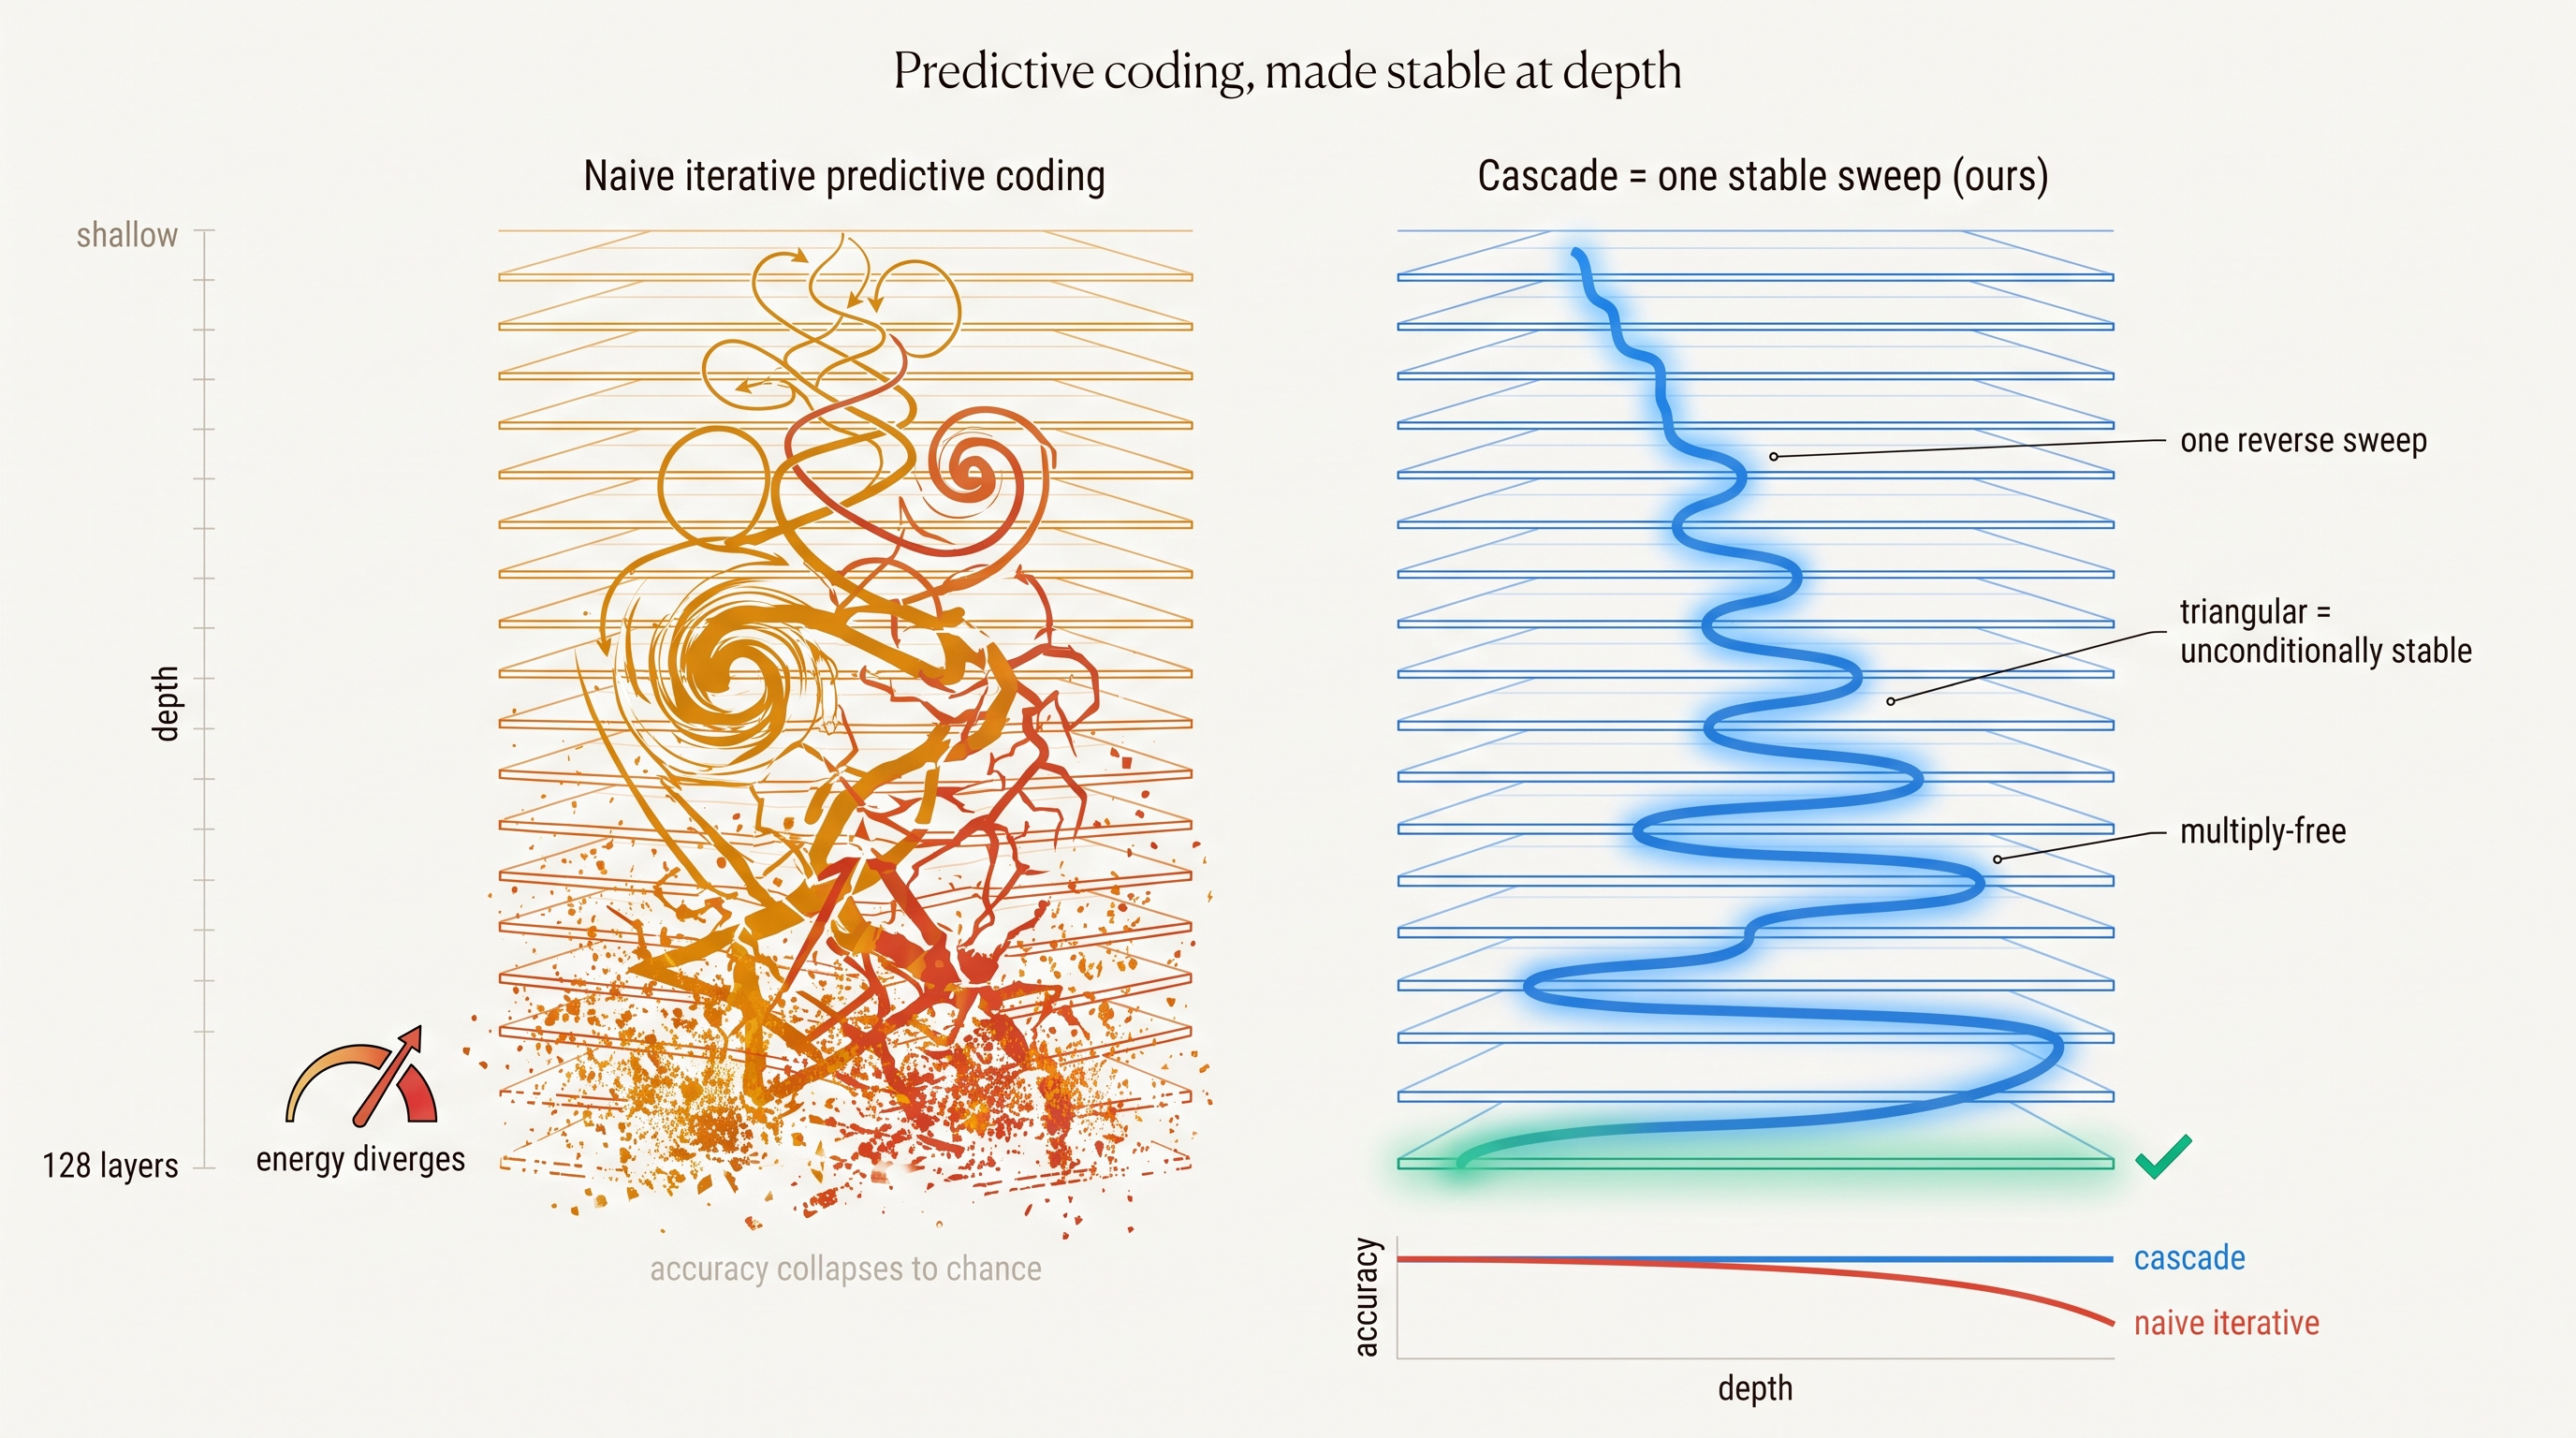
\includegraphics[width=\textwidth]{figs/gen/supp_depth.jpg}
\caption{\textbf{Why predictive coding stays stable at depth on this substrate.}
Naively settling the states of a deep predictive-coding network amplifies error
with depth: the dynamics diverge and accuracy collapses to chance (left). Our
substrate instead relaxes the \emph{errors} with routing frozen, which is
triangular and therefore unconditionally stable, and collapses to a single
multiply-free reverse sweep that stays accurate to 128 layers (right). This is
the conceptual companion to the measured curves in Fig.~\ref{fig:depth}b.
Conceptual illustration.}
\label{supp:depth}
\end{figure}

\begin{figure}[h!]
\centering
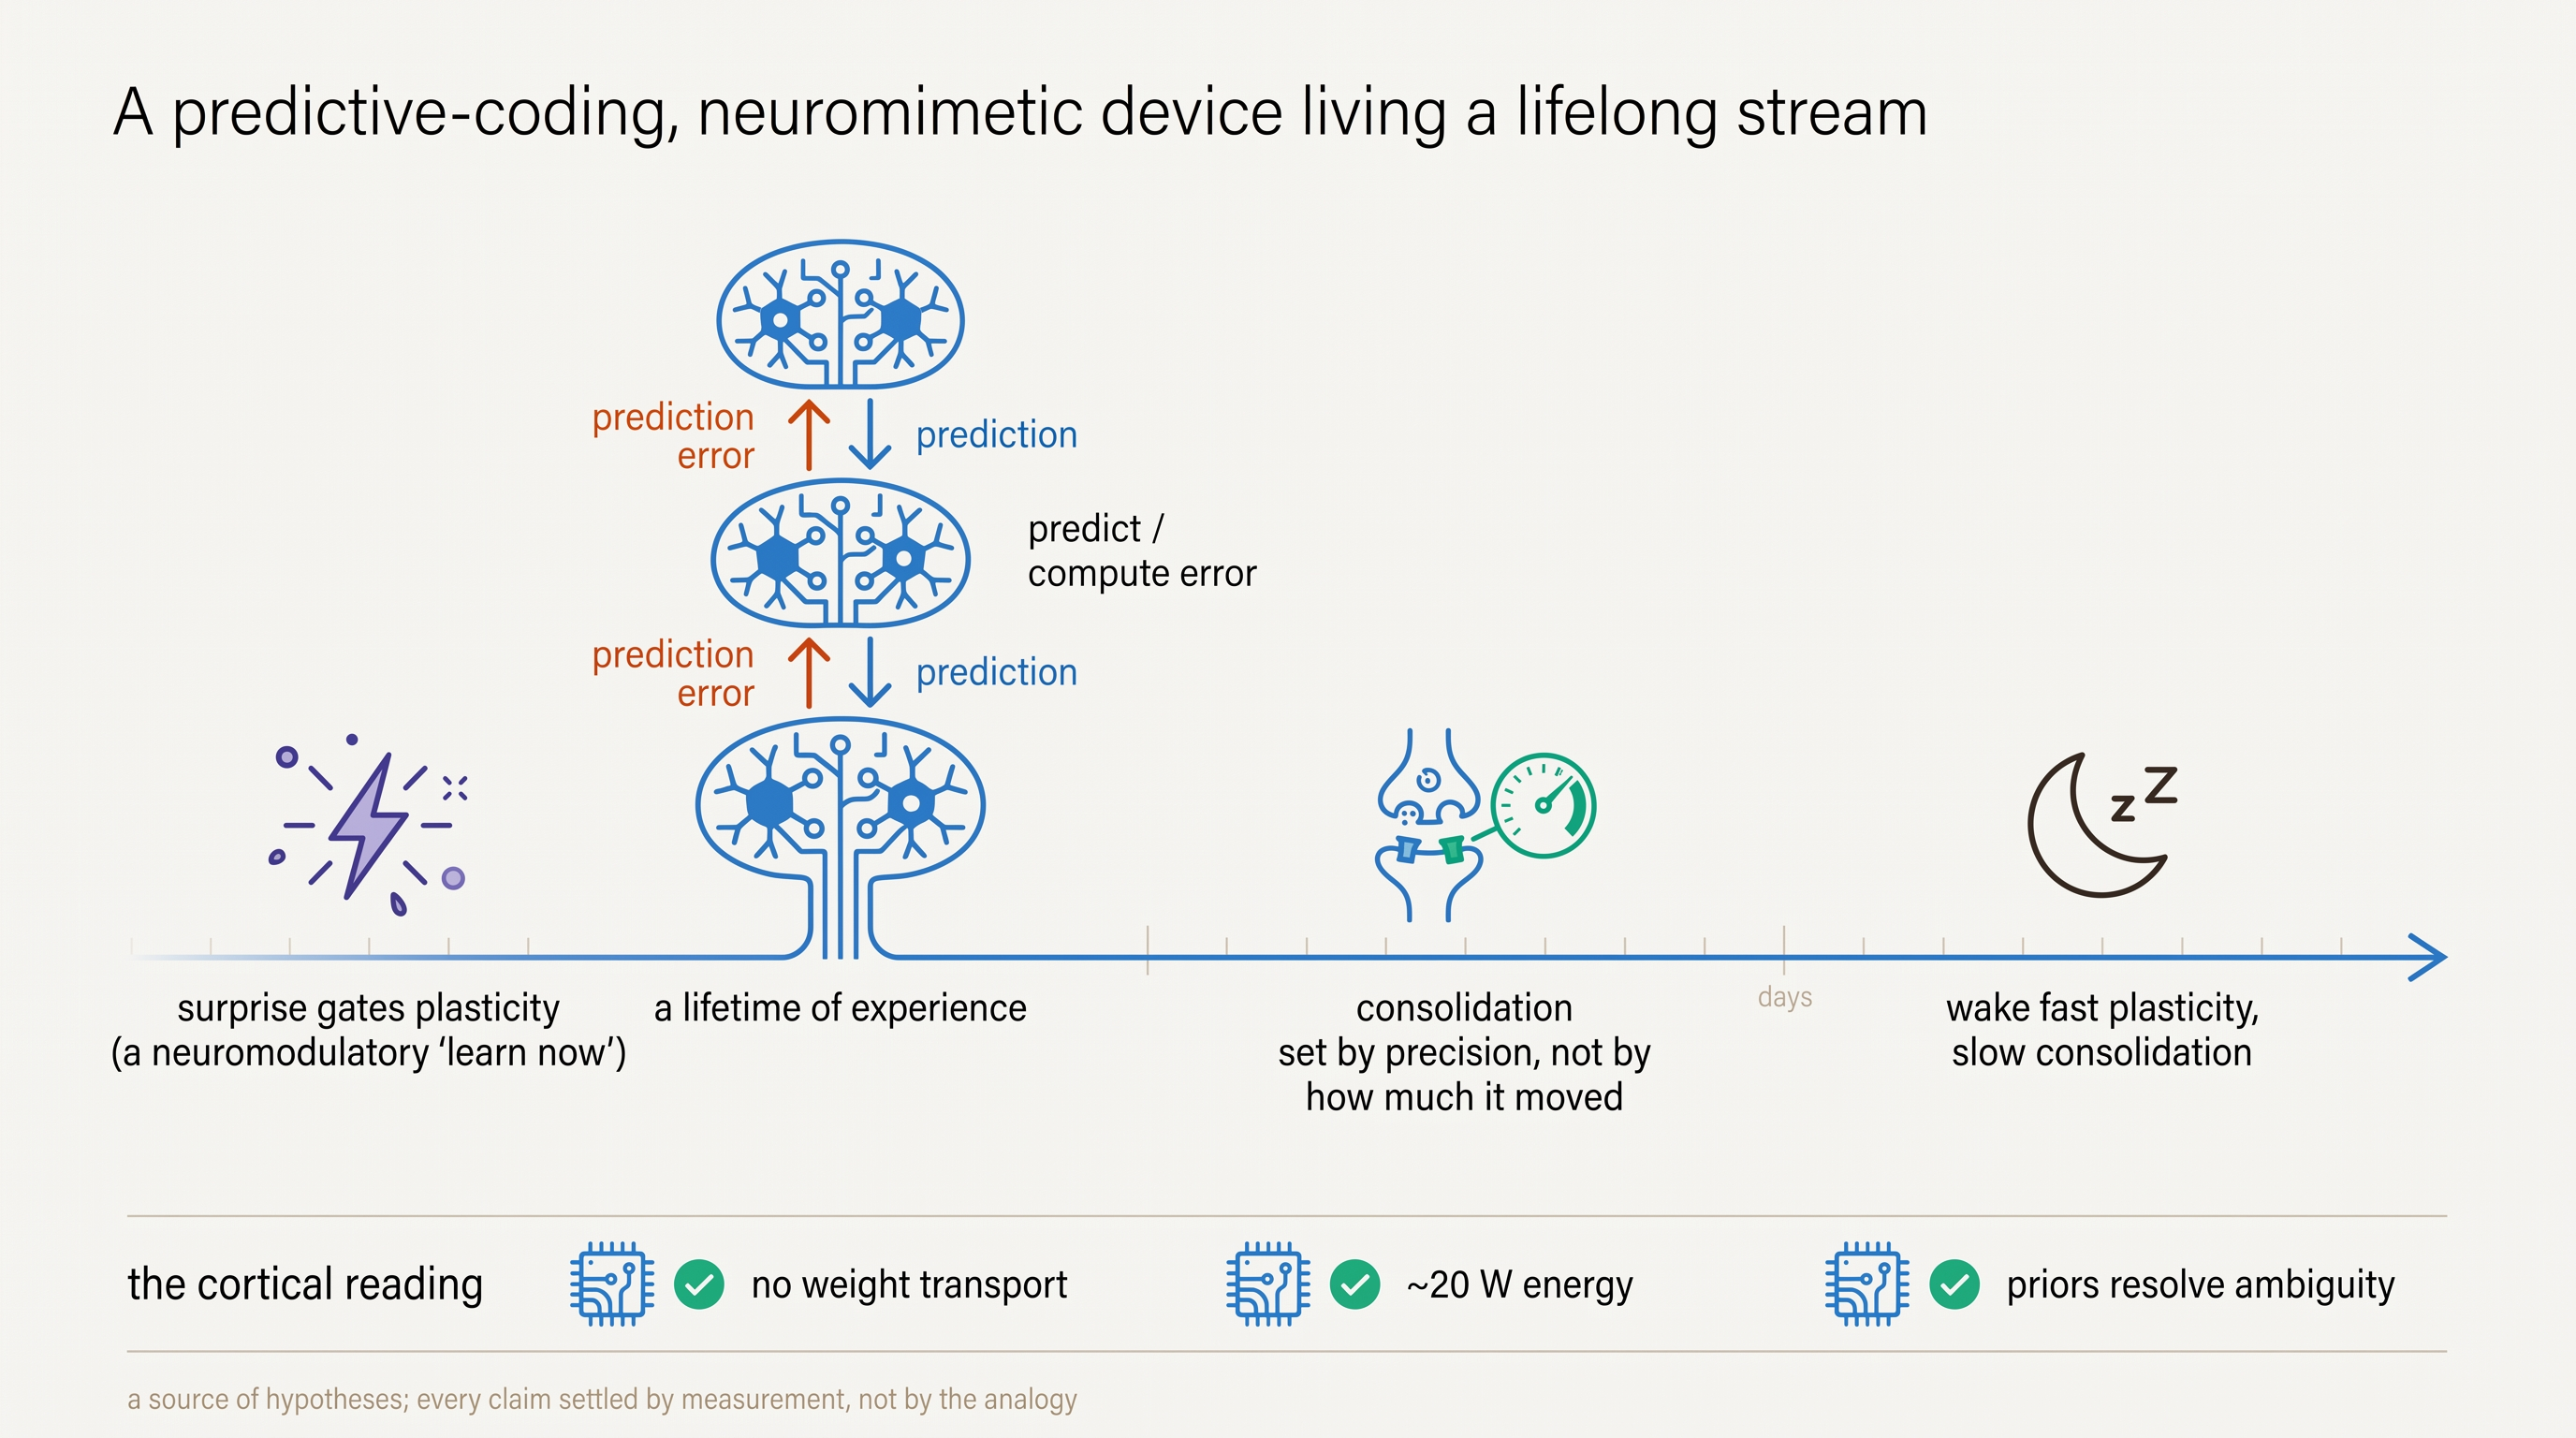
\includegraphics[width=\textwidth]{figs/gen/supp_neuromimetic.jpg}
\caption{\textbf{A predictive-coding, neuromimetic device living a lifelong
stream.} A stylized cortical hierarchy predicts its input and propagates
prediction error; over a lifetime of experience, surprise gates plasticity (a
neuromodulatory ``learn-now'' signal), consolidation is set by the precision of
predictions rather than by the magnitude of change, and fast wake plasticity is
complemented by slow consolidation. The cortical correspondences (no weight
transport, $\sim$20~W energy, priors resolving ambiguity) are a source of
hypotheses; every claim in the paper is settled by measurement, not by the
analogy. \emph{(Design draft; to be redrawn as a vector figure for submission.)}}
\label{supp:neuro}
\end{figure}

\clearpage
\normalsize
\bibliography{references,neuro_refs}

\end{document}
